%============================================================================
% tento soubor pouzijte jako zaklad
% (c) 2008 Michal Bidlo
% E-mail: bidlom AT fit vutbr cz
%============================================================================
% kodovaní: UTF-8 (zmena prikazem iconv, recode nebo cstocs)
%----------------------------------------------------------------------------
% zpracování: make, make pdf, make desky, make clean
%============================================================================
% Šablonu upravil: Ing. Jaroslav Dytrych, idytrych@fit.vutbr.cz
%============================================================================
\documentclass[]{fitthesis} % bez zadání - pro začátek práce, aby nebyl problém s překladem
%\documentclass[zadani]{fitthesis} % odevzdani do wisu - odkazy jsou barevné
%\documentclass[zadani,print]{fitthesis} % pro tisk - odkazy jsou černé
%\documentclass[english,print]{fitthesis} % pro tisk - odkazy jsou černé
% * Je-li prace psana v anglickem jazyce, je zapotrebi u tridy pouzit
%   parametr english nasledovne:
%      \documentclass[english]{fitthesis}
% * Je-li prace psana ve slovenskem jazyce, je zapotrebi u tridy pouzit
%   parametr slovak nasledovne:
%      \documentclass[slovak]{fitthesis}

\usepackage[czech,slovak,english]{babel}
\usepackage[utf8]{inputenc} %kodovani
\usepackage[T1]{fontenc}
\usepackage{cmap}
\usepackage{url}
\DeclareUrlCommand\url{\def\UrlLeft{<}\def\UrlRight{>} \urlstyle{tt}}

%zde muzeme vlozit vlastni balicky
\usepackage{listingsutf8}

\lstset{
    basicstyle=\ttfamily\small,
    escapeinside={(*}{*)},
    numbers=none,
    mathescape,
    breaklines=true,
    breakatwhitespace=true,
    framextopmargin=2pt,
    framexbottommargin=2pt,
    extendedchars=false,
    inputencoding=utf8
}

\usepackage{caption}
\usepackage{hhline}
\usepackage{graphicx}
\usepackage{amsthm}
\usepackage{amssymb}
\usepackage{thmtools}
\usepackage{float}
\usepackage{amsmath}
\usepackage{changepage}
\usepackage{lipsum}
\usepackage{multirow}
\usepackage{tabularx}
\usepackage{courier}
\usepackage{tikz}
\usepackage{calc}

\usepackage[vlined, ruled, czech, linesnumbered, resetcount, algochapter]{algorithm2e}
\usepackage[caption = false]{subfig}


\newcommand{\term}[1]{\textit{#1}}
\newcommand{\symb}[1]{\hspace{0.5mm}\tikz[overlay]\node[fill=gray!10, minimum height=1.2em , draw=gray!20, inner sep=1.5pt, anchor=text, rectangle, rounded corners=1mm]{\texttt{#1}};\phantom{\texttt{#1}}\hspace{0.5mm}}

\SetKw{And}{and}
\SetKw{Or}{or}

\theoremstyle{definition}
\declaretheorem[name=Definice,numberwithin=section,qed={\lower0.3ex\hbox{$\blacktriangle$}}]{defn}
\declaretheorem[name=Příklad,numberwithin=section,qed={\lower0.3ex\hbox{$\blacksquare$}}]{exmp}


\usepackage{listings}
\usepackage[toc,page,header]{appendix}
\RequirePackage{titletoc}
\ifczech
  \usepackage{ae}
\fi


%---rm---------------
\renewcommand{\rmdefault}{lmr}%zavede Latin Modern Roman jako rm
%---sf---------------
\renewcommand{\sfdefault}{qhv}%zavede TeX Gyre Heros jako sf
%---tt------------
\renewcommand{\ttdefault}{lmtt}% zavede Latin Modern tt jako tt

%-----------------------------------------------------------------------------


% Níže jsou deklarace fontů pro testování a ladění JVS 
% - doporučuje se NEPOUŽÍVAT
% Deklarace nejsou doladěné !!!
% Times New Roman není dle JVS povolený (je tu na ukázku)
%-----------------------------------------------------------------------------

\ifOPEN
  \pdfmapfile{=OpenSansfontspdf.map}
  \DeclareFontFamily{T1}{OpenSans}{}
  \DeclareFontShape{T1}{OpenSans}{b}{n}{<->recOpenSans-Bold}{}
  \DeclareFontShape{T1}{OpenSans}{b}{it}{<->recOpenSans-BoldItalic}{}
  \DeclareFontShape{T1}{OpenSans}{eb}{n}{<->recOpenSans-ExtraBold}{}
  \DeclareFontShape{T1}{OpenSans}{eb}{it}{<->recOpenSans-ExtraBoldItalic}{}
  \DeclareFontShape{T1}{OpenSans}{m}{it}{<->recOpenSans-Italic}{}
  \DeclareFontShape{T1}{OpenSans}{l}{n}{<->recOpenSans-Light}{}
  \DeclareFontShape{T1}{OpenSans}{l}{it}{<->recOpenSans-LightItalic}{}
  \DeclareFontShape{T1}{OpenSans}{m}{n}{<->recOpenSans-Regular}{}
  \DeclareFontShape{T1}{OpenSans}{sb}{n}{<->recOpenSans-Semibold}{}
  \DeclareFontShape{T1}{OpenSans}{sb}{it}{<->recOpenSans-SemiboldItalic}{}
  \renewcommand{\rmdefault}{OpenSans}
  \renewcommand{\sfdefault}{OpenSans}
\else
  \iftoggle{declare_open}{
    \pdfmapfile{=OpenSansfontspdf.map}
    \DeclareFontFamily{T1}{OpenSans}{}
    \DeclareFontShape{T1}{OpenSans}{b}{n}{<->recOpenSans-Bold}{}
    \DeclareFontShape{T1}{OpenSans}{b}{it}{<->recOpenSans-BoldItalic}{}
    \DeclareFontShape{T1}{OpenSans}{eb}{n}{<->recOpenSans-ExtraBold}{}
    \DeclareFontShape{T1}{OpenSans}{eb}{it}{<->recOpenSans-ExtraBoldItalic}{}
    \DeclareFontShape{T1}{OpenSans}{m}{it}{<->recOpenSans-Italic}{}
    \DeclareFontShape{T1}{OpenSans}{l}{n}{<->recOpenSans-Light}{}
    \DeclareFontShape{T1}{OpenSans}{l}{it}{<->recOpenSans-LightItalic}{}
    \DeclareFontShape{T1}{OpenSans}{m}{n}{<->recOpenSans-Regular}{}
    \DeclareFontShape{T1}{OpenSans}{sb}{n}{<->recOpenSans-Semibold}{}
    \DeclareFontShape{T1}{OpenSans}{sb}{it}{<->recOpenSans-SemiboldItalic}{}
  }
\fi


\ifVAFLE
  \pdfmapfile{=Vafle_VUT_fontspdf.map}
  \DeclareFontFamily{T1}{VafleVUT}{}
  \DeclareFontShape{T1}{VafleVUT}{m}{n}{<->recVafle_VUT_Regular}{}
  \DeclareFontShape{T1}{VafleVUT}{b}{n}{<->recVafle_VUT_Bold}{}
  \DeclareFontShape{T1}{VafleVUT}{l}{n}{<->recVafle_VUT_Light}{}
  \renewcommand{\rmdefault}{VafleVUT}
  \renewcommand{\sfdefault}{VafleVUT}
  % Tohle je škaredý hack - Vafle nemá it a když se s tím nic neudělá, kurzíva
  % se nijak neprojeví (jen varováním při překladu). Nicméně "doplňkový" font 
  % OpenSans kurzívu má a v semibold to dle mého názoru vypadá pro demonstrační
  % účely při ladění JVS přijatelně.
  \let\oldit\it
  \renewcommand{\it}{\usefont{T1}{OpenSans}{sb}{it}}
\else
  \ifTVAFLE
    \pdfmapfile{=Vafle_VUT_fontspdf.map}
    \DeclareFontFamily{T1}{VafleVUT}{}
    \DeclareFontShape{T1}{VafleVUT}{m}{n}{<->recVafle_VUT_Regular}{}
    \DeclareFontShape{T1}{VafleVUT}{b}{n}{<->recVafle_VUT_Bold}{}
    \DeclareFontShape{T1}{VafleVUT}{l}{n}{<->recVafle_VUT_Light}{}
    \pdfmapfile{=OpenSansfontspdf.map}
    \DeclareFontFamily{T1}{OpenSans}{}
    \DeclareFontShape{T1}{OpenSans}{b}{n}{<->recOpenSans-Bold}{}
    \DeclareFontShape{T1}{OpenSans}{b}{it}{<->recOpenSans-BoldItalic}{}
    \DeclareFontShape{T1}{OpenSans}{eb}{n}{<->recOpenSans-ExtraBold}{}
    \DeclareFontShape{T1}{OpenSans}{eb}{it}{<->recOpenSans-ExtraBoldItalic}{}
    \DeclareFontShape{T1}{OpenSans}{m}{it}{<->recOpenSans-Italic}{}
    \DeclareFontShape{T1}{OpenSans}{l}{n}{<->recOpenSans-Light}{}
    \DeclareFontShape{T1}{OpenSans}{l}{it}{<->recOpenSans-LightItalic}{}
    \DeclareFontShape{T1}{OpenSans}{m}{n}{<->recOpenSans-Regular}{}
    \DeclareFontShape{T1}{OpenSans}{sb}{n}{<->recOpenSans-Semibold}{}
    \DeclareFontShape{T1}{OpenSans}{sb}{it}{<->recOpenSans-SemiboldItalic}{}
  \fi
\fi

\ifARIAL
  \pdfmapfile{=arialfontspdf.map}
  \DeclareFontFamily{T1}{arial}{}
  \DeclareFontShape{T1}{arial}{b}{n}{<->recarialbd}{}
  \DeclareFontShape{T1}{arial}{b}{sl}{<->recarialbdo}{}
  \DeclareFontShape{T1}{arial}{b}{it}{<->recarialbi}{}
  \DeclareFontShape{T1}{arial}{m}{n}{<->recarial}{}
  \DeclareFontShape{T1}{arial}{m}{sl}{<->recarialo}{}
  \DeclareFontShape{T1}{arial}{m}{it}{<->recariali}{}
  \DeclareFontShape{T1}{arial}{bx}{n}{<->ssub * arial/b/n}{}
  \DeclareFontShape{T1}{arial}{bx}{sl}{<->ssub * arial/b/sl}{}
  \DeclareFontShape{T1}{arial}{bx}{it}{<->ssub * arial/b/it}{}
  \renewcommand{\rmdefault}{arial}
  \renewcommand{\sfdefault}{arial}
\else
  \ifTARIAL
    \pdfmapfile{=arialfontspdf.map}
    \DeclareFontFamily{T1}{arial}{}
    \DeclareFontShape{T1}{arial}{b}{n}{<->recarialbd}{}
    \DeclareFontShape{T1}{arial}{b}{sl}{<->recarialbdo}{}
    \DeclareFontShape{T1}{arial}{b}{it}{<->recarialbi}{}
    \DeclareFontShape{T1}{arial}{m}{n}{<->recarial}{}
    \DeclareFontShape{T1}{arial}{m}{sl}{<->recarialo}{}
    \DeclareFontShape{T1}{arial}{m}{it}{<->recariali}{}
    \DeclareFontShape{T1}{arial}{bx}{n}{<->ssub * arial/b/n}{}
    \DeclareFontShape{T1}{arial}{bx}{sl}{<->ssub * arial/b/sl}{}
    \DeclareFontShape{T1}{arial}{bx}{it}{<->ssub * arial/b/it}{}
  \fi
\fi

\ifTIMES
  \pdfmapfile{=timesfontspdf.map}
  \DeclareFontFamily{T1}{times}{}
  \DeclareFontShape{T1}{times}{m}{n}{<->rectimes}{}
  \DeclareFontShape{T1}{times}{m}{it}{<->rectimesi}{}
  \DeclareFontShape{T1}{times}{b}{n}{<->rectimesbd}{}
  \DeclareFontShape{T1}{times}{b}{it}{<->rectimesbi}{}
  \renewcommand{\rmdefault}{times}
  \renewcommand{\sfdefault}{times}
\fi


% vypne funkci nové šablony, která automaticky nahrazuje uvozovky,
% aby nebyly prováděny nevhodné náhrady v popisech API apod.
\csdoublequotesoff

% =======================================================================
% balíček "hyperref" vytváří klikací odkazy v pdf, pokud tedy použijeme pdflatex
% problém je, že balíček hyperref musí být uveden jako poslední, takže nemůže
% být v šabloně
\ifWis
\ifx\pdfoutput\undefined % nejedeme pod pdflatexem
\else
  \usepackage{color}
  \usepackage[unicode,colorlinks,hyperindex,plainpages=false,pdftex]{hyperref}
  \definecolor{links}{rgb}{0.4,0.5,0}
  \definecolor{anchors}{rgb}{1,0,0}
  \def\AnchorColor{anchors}
  \def\LinkColor{links}
  \def\pdfBorderAttrs{/Border [0 0 0] }  % bez okrajů kolem odkazů
  \pdfcompresslevel=9
\fi
\else % pro tisk budou odkazy, na které se dá klikat, černé
\ifx\pdfoutput\undefined % nejedeme pod pdflatexem
\else
  \usepackage{color}
  \usepackage[unicode,colorlinks,hyperindex,plainpages=false,pdftex,urlcolor=black,linkcolor=black,citecolor=black]{hyperref}
  \definecolor{links}{rgb}{0,0,0}
  \definecolor{anchors}{rgb}{0,0,0}
  \def\AnchorColor{anchors}
  \def\LinkColor{links}
  \def\pdfBorderAttrs{/Border [0 0 0] } % bez okrajů kolem odkazů
  \pdfcompresslevel=9
\fi
\fi

%Informace o praci/projektu
%---------------------------------------------------------------------------
\projectinfo{
  %Prace
  project=BP,            %typ prace BP/SP/DP/DR
  year=2016,             %rok
  date=\today,           %datum odevzdani
  %Nazev prace
  title.csnl={Syntaktická analýza založená\newline na gramatikách řízených stromy},  %nazev prace v cestine se zalomenim
  title.cs={Syntaktická analýza založená na gramatikách řízených stromy},  %nazev prace v cestine
  title.en={Parsing Based on Tree-Controled Grammars}, %nazev prace v anglictine
  %Autor
  author={Štěpán Granát},   %cele jmeno a prijmeni autora
  author.name={Štěpán},   %jmeno autora (pro citaci)
  author.surname={Granát},   %prijmeni autora (pro citaci)
  %author.title.p=Bc., %titul pred jmenem (nepovinne)
  %author.title.a=PhD, %titul za jmenem (nepovinne)
  %Ustav
  department=UIFS, % doplnte prislusnou zkratku dle ustavu na zadani: UPSY/UIFS/UITS/UPGM
  %Skolitel
  supervisor={Alexander Meduna}, %cele jmeno a prijmeni skolitele
  supervisor.name={Alexander},   %jmeno skolitele (pro citaci)
  supervisor.surname={Meduna},   %prijmeni skolitele (pro citaci)
  supervisor.title.p={Prof. RNDr.},   %titul pred jmenem (nepovinne)
  supervisor.title.a={CSc.},    %titul za jmenem (nepovinne)
  %Klicova slova, abstrakty, prohlaseni a podekovani je mozne definovat
  %bud pomoci nasledujicich parametru nebo pomoci vyhrazenych maker (viz dale)
  %===========================================================================
  %Klicova slova
  %keywords.cs={Klíčová slova v českém jazyce.}, %klicova slova v ceskem ci slovenskem jazyce
  %keywords.en={Klíčová slova v anglickém jazyce.}, %klicova slova v anglickem jazyce
  %Abstract
  %abstract.cs={Výtah (abstrakt) práce v českém jazyce.}, % abstrakt v ceskem ci slovenskem jazyce
  %abstract.en={Výtah (abstrakt) práce v anglickém jazyce.}, % abstrakt v anglickem jazyce
  %Prohlaseni
  %declaration={Prohlašuji, že jsem tuto bakalářskou práci vypracoval samostatně pod vedením pana ...},
  %Podekovani (nepovinne)
  %acknowledgment={Zde je možné uvést poděkování vedoucímu práce a těm, kteří poskytli odbornou pomoc.} % nepovinne
}

%Abstrakt (cesky, slovensky ci anglicky)
\abstract[cs]{Cílem této práce je navrhnout a implementovat syntaktický analyzátor
    gramatik, jejichž derivační strom je omezen pomocí kontroly úrovní.
    Běžné postupy syntaktické analýzy jsou podrobně rozebrány a
    poté je diskutováno, jak by mohly být rozšířeny o kontrolu
    derivačního stromu.
    Nejdůležitější částí práce je návrh
    průběžné kontroly derivačního stromu souběžně s jeho konstrukcí,
    což umožňuje úzké propojení těchto dvou procesů.
    Uvedený přístup přináší výrazné zvýšení síly syntaktického analyzátoru.}

\abstract[en]{The goal of this thesis is to design and implement the parser
    of grammars, whose derivation tree is limited by inspection of levels.
    Common parsing procedures are studied in detail and then it is discussed,
    how they could be extended by inspection of derivation tree.
    The most important part of the thesis is a draft of continuous inspection
    of the derivation tree simultaneously with its construction,
    which allows close cooperation between these two processes.
    This approach enables significant increasing of the parser power.
  }

%Klicova slova (cesky, slovensky ci anglicky)
\keywords[cs]{gramatiky řízené stromy, syntaktická analýza, bezkontextové gramatiky}
\keywords[en]{tree controlled grammars, syntactic analysis, context-free grammars}

%Prohlaseni (u anglicky psane prace anglicky, u slovensky psane prace slovensky)
\declaration{Prohlašuji, že jsem tuto bakalářskou práci vypracoval samostatně pod vedením profesora RNDr. Alexandera Meduny, CSc.
Uvedl jsem všechny literární prameny a publikace, ze kterých jsem čerpal.}

%Podekovani (nepovinne, nejlepe v jazyce prace)
\acknowledgment{Děkuji prof. Alexanderu Medunovi za ochotu vést tuto práci, jeho odborné rady a morální podporu.}

\begin{document}
  % Vysazeni titulnich stran
  % ----------------------------------------------
  \maketitle
  % Obsah
  % ----------------------------------------------
  \tableofcontents

  % Seznam obrazku a tabulek (pokud prace obsahuje velke mnozstvi obrazku, tak se to hodi)
\ifczech
  \renewcommand\listfigurename{Seznam obrázků}
\fi
\ifslovak
  \renewcommand\listfigurename{Zoznam obrázkov}
\fi

  % \listoffigures
\ifczech
  \renewcommand\listtablename{Seznam tabulek}
\fi
\ifslovak
  \renewcommand\listtablename{Zoznam tabuliek}
\fi

  % \listoftables

  % Text prace
  % ----------------------------------------------
  % !TEX root = ./projekt.tex
%=========================================================================
% (c) Michal Bidlo, Bohuslav Křena, 2008

\chapter{Úvod}

\chapter{Definice a pojmy}

Tato práce předpokládá, že je čtenář seznámen s \term{Teorií grafů} a
se základy \term{Teorie formálních jazyků} (viz. \cite{MedunaIFJ}).
Uvedeny jsou jen definice, jež jsou zásadní pro pozdější výklad.

\begin{defn}
  (Strom)\\
  \term{Strom} je orientovaný acyklický graf, $G = (\Sigma, R)$, který má tyto
  tři vlastnosti:
  \begin{itemize}
    \item   $G$ má právě jeden uzel, do něhož nevstupují žádné hrany;
      tento uzel se nazývá kořen $G$ označovaný jako kořen($G$).
    \item Jestliže $a \in \Sigma$ a $a \neq$ kořen($G$), potom $a$ je
    potomkem kořenu($G$) a vstupuje do něj právě jedna hrana.
    \item   Každý uzel $a \in \Sigma$ který není listem má svého přímého potomka,
      $b_1$ až $b_n$, řazené zleva doprava tak, že $b_1$ je
      nejlevějším přímým potomkem $a$ a $b_n$ je nejpravějším přímým
      potomkem $a$.
  \end{itemize}
  \vspace{-0.5cm}
\end{defn}

\begin{defn}
  (Úroveň, cesta, hranice, hloubka, elementární strom a podstrom)\\
  Nechť $G = (\Sigma, R)$ je stromem.
  \begin{itemize}
    \item \term{Úroveň} $l$, stromu $G$, je posloupnost $s$,
      všech uzlů se stejnou vzdáleností od kořene($G$).
      Jinými slovy, úroveň $l$, je posloupnost, $s = n_1 n_2 ... n_k$,
      taková, že existuje cesta v grafu o délce $\ell$ v $G$
      pro všechny posloupnost od kořene($G$)
      $ ... n_i$, pro $1 \leq i \leq k$ a $l \geq 1$.

    \item \term{Cesta} $p$, stromu $G$, je posloupnost $s$, uzlů,
      kde první uzel je kořen($G$), poslední je listem a mezi každými
      dvěma následnými uzly v $s$ existuje hrana v $G$.
      Jinými slovy, cesta $p$ stromu $G$, je posloupnost,
      $s = n_1 n_2 ... n_k$, taková, že $s$ je cesta grafem
      o délce $k$ v $G$, kde $n_1 =$ kořen($G$) a $n_k$ je listem
      v $G$, pro $k \geq 1$.

    \item \term{Hranice} stromu $G$, hranice($G$),
      je posloupnost listů $G$ řazených zleva do prava.

    \item \term{Hloubka} stromu $G$, hloubka($G$), je délka nejdelší cesty v $G$;
      jestliže platí hloubka($G$)$ = 1$, potom je $G$ elementární strom.

    \item Jestliže $G' = (\Sigma', R')$ představuje strom vyhovující těmto
      čtyřem podmínkám:
      $\Sigma' \neq \emptyset$;
      $\Sigma' \subseteq \Sigma$;
      $R' = (\Sigma' \times \Sigma')$;
      a jestliže v $G$ není žádný z uzlů v $\Sigma - \Sigma'$ potomkem
      uzlu v $\Sigma'$, potom je $G'$ \term{podstromem} $G$.
  \end{itemize}
  \vspace{-0.5cm}
\end{defn}

\chapter{Formální jazyky}

Teorie formálních jazyků formalizuje pojmy spojené s jazyky
(přirozenými, programovacími, matematickými, ...), abychom se mohli zabývat
jejich automatizovaným zpracováním.
Pojmy, které známe z lingvistiky jsou zde zobecněny a přesně definovány,
takže nemusí úplně odpovídat tomu, jak jsou chápány v jiných vědních oborech.

\subsubsection*{Abeceda}

Základem jazyka je \term{abeceda}. V teorii formálních jazyků je obvykle značena
$\Sigma$ (sigma) a je definována jako konečná neprázdná množina, jejíž objekty
se nazývají \term{symboly}.

\subsubsection*{Řetězec}

Konečná posloupnost symbolů patřících do $\Sigma$ je \term{řetězec} nad $\Sigma$.
Zvláštním případem je $\varepsilon$ (epsilon), značící \term{prázdný řetězec} -
tedy takový, že neobsahuje žádný symbol.

\subsubsection*{Jazyk}

$\Sigma^*$ značí množinu všech řetězců, které je možné sestrojit nad abecedou $\Sigma$.
Jakákoliv podmnožina $L \subseteq \Sigma^*$ je \term{jazykem} nad abecedou $\Sigma$.
Jestliže \term{jazyk} představuje konečnou množinu řetězců, potom jej nazýváme \term{konečným jazykem},
v opačném případě \term{jazykem nekonečným}.

\subsubsection*{Gramatika}

Pokud se zabýváme nekonečnými jazyky, nemůžeme je vyjádřit jednoduchým výčtem jejich
řetězců. Místo toho definujeme \term{gramatiku}, která stanovuje pravidla pro generování
řetězců patřících do daného jazyka.\\

\noindent
\term{Gramatika} obsahuje 4 části:
\begin{itemize}
  \item Množinu \term{neterminálních symbolů} $N$ (\term{neterminálů}), které slouží k označení syntaktických celků.
  \item Množinu \term{terminálních symbolů} $\Sigma$ (\term{terminálů}) - symboly, které jsou konečným výstupem. (abeceda)
  \item Množinu \term{přepisovacích pravidel} $P$.
  \item Počáteční (startovací) symbol $S \in N$.
\end{itemize}

\subsubsection*{Přepisovací pravidla}
\label{term:rewriteRule}

\term{Přepisovací pravidlo} je složeno ze dvou řetězců $(\alpha, \beta)$,
složených z terminálů a neterminálů, přičemž $\alpha$ obsahuje alespoň jeden \term{neterminál}.
Zapisují se jako $\alpha \rightarrow \beta$.\\
Pravidla se aplikují od počátčního symbolu, kdy postupně přepisujeme řetězec tak že nahradíme
jakoukoliv část řetězce, která se nachází na levé straně některého pravidla za pravou stranu tohoto pravidla.
Tato operace se také nazývá \term{derivace}.
Řetězec upravujeme podle pravidel tak dlouho, až se v něm nacházejí pouze \term{terminály}.

\begin{figure}[H]
  \centering
  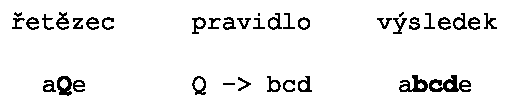
\includegraphics{fig/rewriteRule.pdf}
  \caption{Příklad derivace podle pravidla}
  \label{img:rewriteRule}
\end{figure}

\subsubsection*{Ekvivalence gramatik}
Dvě gramatiky označujeme jako \term{ekvivalentní}, pokud generují stejný jazyk.

\subsubsection*{Výpočetní model}

\term{Výpočetní model} lze definovat jako hypotetický přístroj,
který obsahuje množinu povolených operací. Povolené operace modelu určují,
jak sofistikované problémy je schopen řešit.

\subsubsection*{Hierarchie jazyků}
\label{subsec:chomHierarchy}

Omezením gramatiky lze zaručit to, že ji lze zpracovávat jednodušším
\term{výpočetním modelem}. Jazyky se proto
dělí do tříd právě podle toho, jaký výpočetní model je dokáže zpracovat.\\

\noindent
Jedno z nejznámějších rozdělení je podle tzv. \term{Chomského hierarchie}:

\begin{itemize}
  \item \textbf{Gramatiky typu 0} (frázové/neomezené gramatiky)\\
  Zahrnují všechny formální gramatiky.\\
  Model pro zpracování se nazývá \term{Turingův stroj}.\\
  Tvoří třídu \term{rekurzivně spočetných jazyků}, zkratka \textbf{RE}.

  \item \textbf{Gramatiky typu 1} (kontextové gramatiky)\\
  Tyto gramatiky se skládají z pravidel typu $\alpha A\beta \rightarrow \alpha \gamma \beta$,
  kde $A$ je neterminál a $\alpha, \beta, \gamma$ jsou řetězce terminálů i neterminálů,
  přičemž $\gamma$ je neprázdný.\\
  Model pro zpracování se nazývá \term{lineárně ohraničený Turingův stroj}.\\
  Tvoří třídu \term{kontextových jazyků}, zkratka \textbf{CS}.

  \item \textbf{Gramatiky typu 2} (bezkontextové gramatiky)\\
  Skládají se z pravidel typu $A \rightarrow \gamma$, kde $A$ je neterminál a
  $\gamma$ řetězec terminálů a neterminálů.\\
  Model pro zpracování se nazývá \term{nedeterministický zásobníkový automat}.\\
  Tvoří třídu \term{bezkontextových jazyků}, zkratka \textbf{CF}.

  \item \textbf{Gramatiky typu 3} (regulární gramatiky)\\
  Skládají se z pravidel typu $A \rightarrow B$ a $A \rightarrow aB$,
  kde $A, B$ jsou neterminály a $a$ je terminál.\\
  Model pro zpracování se nazývá \term{konečný automat}.\\
  Tvoří třídu \term{regulárních jazyků}, zkratka \textbf{REG}.
\end{itemize}

\subsubsection*{Vyjadřovací síla jazyka}

Čím větší má jazyk vyjadřovací sílu, tím detailnější omezení je jeho
gramatika schopna klást na přijímané řetězce. Jsme tedy schopni jemněji rozlišovat,
které řetězce patří do jazyka a které ne.

V \term{Chomského hierarchii} jsou jazyky uspořádány tak, že slabší jazyk je
vždy podmnožinou silnějšího. Tedy například mezi Bezkontextové jazyky patří i
všechny Regulární jazyky.\\

\begin{figure}[H]
  \centering
  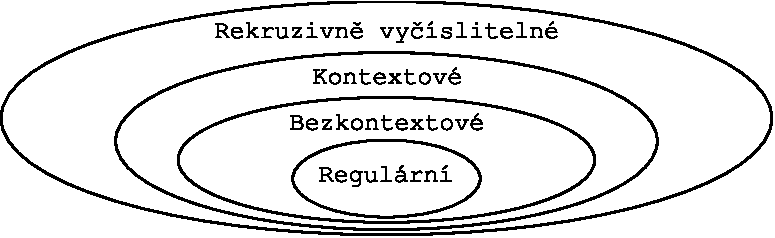
\includegraphics{fig/Chomsky.pdf}
  \caption{Schématické znázornění Chomského hieararchie}
\end{figure}

\section{Regulární jazyky}

Regulární jazyky jsou nejjednodušší formální jazyky v Chomského hierarchii.
I přesto si však našly široké využití v různých oblastech informačních technologií.
Využívají se např. pro pokročilé vyhledávání v textu nebo
pro rozdělení programovacího jazyka na základní jednotky.
V implementační části této práce jsou využity ke kontrole úrovní derivačního stromu,
také proto se jimi budeme hlouběji zabývat.

\begin{defn}
  (Regulární jazyk)\\
  \term{Regulární jazyk} nad abecedou $\Sigma$ lze definovat následovně:
  \begin{itemize}
    \item Prázdný jazyk $\emptyset$ je regulární.
    \item Pro každé $a$ z $\Sigma$ je $\{ a \}$ regulární.
    \item Jestliže $A$ a $B$ jsou regulární jazyky, poté všechny tyto jazyky jsou také regulární:
    $A \cup B$ (sjednocení), $AB$ (konkatenace) a $A^*$ (iterace).
  \end{itemize}
\end{defn}

\subsection{Konečné automaty}
Každý Regulární jazyk lze zpracovávat konečným automatem a každý konečný automat
lze vyjádřit regulárním jazykem.\\


\begin{defn} (Konečný automat)\\
  \term{Konečný automat} je pětice $M = (Q, \Sigma, R, s, F)$, kde:
  \begin{itemize}
    \item $Q$ je množina stavů
    \item $\Sigma$ je \term{vstupní abeceda}
    \item $R$ je množina \term{přechodových pravidel}
    \item $s$ je \term{počáteční stav}
    \item $F$ je množina \term{konečných stavů}
  \end{itemize}
\end{defn}

Přechodová pravidla jsou ve tvaru $qa \rightarrow p$, kde $q, p$ jsou stavy a
$a$ je vstupní symbol. Pravidlo nám říká, že jsme-li ve stavu $q$ a na vstupu
máme symbol $a$, poté může automat přejít do stavu $p$.
Začínáme vždy v počátečním stavu a aby vstupní řetězec patřil do jazyka,
musíme skončit v jednom z konečných stavů.
Velkou výhodou je, že práce konečného automatu je paměťově velmi nenáročná,
jelikož obsahuje pouze informaci o aktuálním stavu.

\begin{exmp}
  Mějme konečný automat M1:
  \begin{lstlisting}
  M1 = (
    {s, q, f},        (* // množina stavů *)
    {a, b, c},        (* // abeceda *)
    {                 (* // množina pravidel *)
      sa $\rightarrow$ q1,
      qb $\rightarrow$ q,
      qc $\rightarrow$ f
    },
    s,                (* // počateční stav *)
    {f}               (* // množina ukončujících stavů *)
  )
  \end{lstlisting}
  A řetězec:
\begin{lstlisting}
  abbc
\end{lstlisting}

\noindent
Při kontrole vstupního řetězce budeme postupovat následovně:

\begin{enumerate}
  \item Nastavíme počáteční stav $s$
  \item Vstupním symbolem je \symb{a} - podle prvního pravidla přejdeme do stavu $q$
  \item Vstupním symbolem je \symb{b} - zůstáváme ve stavu $q$ (pr. 2)
  \item Vstupním symbolem je \symb{b} - zůstáváme ve stavu $q$ (pr. 2)
  \item Vstupním symbolem je \symb{c} - přejdeme do stavu $f$ (pr. 3)
  \item Jsme na konci řetězce - zkontrolujeme, zdali jsme v konečném stavu - řetězec byl automatem přijat,
  takže řetězec patří do jazyka generovaného automatem.
\end{enumerate}

\noindent
Během činnosti konečného automatu mohou nastat tyto chyby:

\begin{itemize}
  \item vstupní symbol nepatří do abecedy
  \item neexistuje pravidlo pro vstupní symbol a aktuální stav
  \item po přečtení posledního znaku se nenacházíme v konečném stavu
\end{itemize}
Ve všech těchto případech není vstupní řetězec přijat konečným automatem, tudíž nepatří
do jazyka generovaného automatem.\\

\noindent
Tento konečný automat lze také zobrazit pomocí následujícího grafu:

\begin{figure}[H]
  \centering
  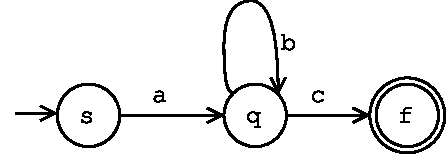
\includegraphics{fig/finiteAutomat.pdf}
\end{figure}

\end{exmp}

\noindent
Uveďme další příklad, který už nebude tak jednoduchý:
\begin{exmp}
  Mějme konečný automat M2:
  \begin{lstlisting}
  M2 = (
    {s, q1, q2, p1, p2, f1, f2},
    {a, b, c, d},
    {
      sa $\rightarrow$ q1,
      q1b $\rightarrow$ q2,
      q2c $\rightarrow$ f1,
      q1$\varepsilon$ $\rightarrow$ p1,
      p1b $\rightarrow$ p2,
      p2d $\rightarrow$ f2
    },
    s1,
    {f1}
  )
  \end{lstlisting}

  Za pozornost stojí hlavně čtvrté pravidlo s $\varepsilon$ přechodem.
  Toto pravidlo značí, že lze bez přijetí jakéhokoliv znaku přejít z jednoho stavu
  do druhého. Tyto pravidla se bohužel mohou v obecných konečných automatech vyskytovat a
  způsobují potíže při zpracovávání automatu, jak bude vysvětleno dále.\\

  \noindent
  Pro větší názornost budeme nyní pracovat se schématem automatu:

  \begin{figure}[H]
    \centering
    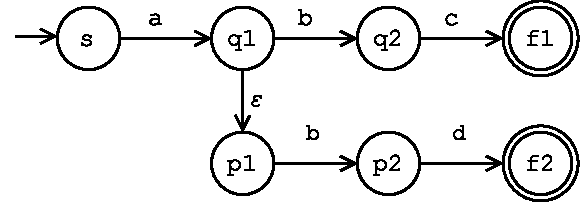
\includegraphics{fig/finiteAutomat1.pdf}
  \end{figure}

  Pokud se při zpracování ocitneme ve stavu $q1$ a vstupním symbolem bude \symb{b},
  není jasné, jestli máme použít 2. nebo 4. pravidlo. Museli bychom vyzkoušet jít oběma cestami
  a až zpětně bychom zjistili, která možnost byla správná. Tomuto jevu se v teorii
  formálních jazyků říká \term{nedeterminismus} a setkáme
  se s ním ještě několikrát.\\
\end{exmp}

  Nutno ale podotknout, že v tomto případě \term{nedeterminismus} neznamená,
  že bychom nebyli schopni
  určit, jestli řetězec patří do daného jazyka. Ve skutečnosti totiž můžeme
  vyzkoušet všechna možná pravidla a zjistit, jestli z nich některé povede k úspěchu.
  Slepé zkoušení pravidel však vede k velkému zpomalení vyhodnocování,
  může totiž dojít k tomu, že se program bude větvit opakovaně
  a délka zpracování bude neúnosná. Požadavek na striktní determinismus
  je tedy hlavně snaha o co nejrychlejší zpracování.


\subsection{Determinizace konečného automatu}

Z výše uvedených odstavců je zjevné, že je lepší se preventivně nedeterminismu
zbavit. Nejprve ukážeme demonstraci na tomto konkrétním příkladě a poté uvedeme
obecný algoritmus.\\

Abychom se zbavili $\varepsilon$ přechodů musíme vytvořit nový automat, který ale
generuje stejný jazyk (přijímá stejné řetězce),
jako ten původní. Takovéto dva automaty se označují jako \term{ekvivalentní}.
Protože můžeme z přechodu $q1$ kdykoliv přejít do $q2$ intuitivním řešením
je oba stavy spojit do jednoho. Pro zachování \term{ekvivalence}, musíme
do nového stavu přidat všechna pravidla, která vycházela z původních dvou stavů.
Nový automat bude vypadat takto:

\begin{figure}[H]
  \centering
  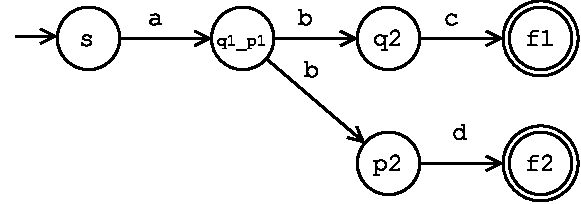
\includegraphics{fig/finiteAutomat1_1.pdf}
\end{figure}

Pokud si nové schéma dobře prohlédneme, odhalíme další zádrhel, který se nám
objevil v novém pravidle $q1\_p1$. Pokud je v tomto stavu na vstupu symbol \symb{b},
nevíme které pravidlo použít a máme tu opět \term{nedeterminismus}.
I tento problém lze naštěstí vyřešit obdobným způsobem:

\begin{figure}[H]
  \centering
  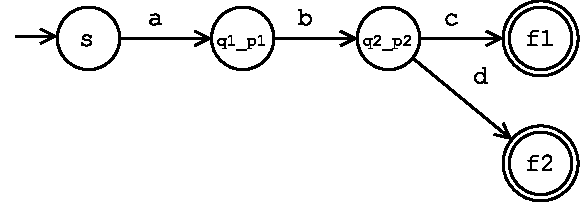
\includegraphics{fig/finiteAutomat1_2.pdf}
\end{figure}

\noindent
Tento automat můžeme označit jako \term{deterministický} a lze jej
s klidem implementovat.

\noindent
V tomto konkrétním případě jsme si pomohli intuicí, uveďme ale obecné algoritmy:\\

\begin{algorithm}[H]
  \caption{Stavy dostupné bez čtení ze stavů $E$ (\term{$\varepsilon$-closure(E)})}
  \KwIn{Končný automat $M = (Q, \Sigma, R, s, F)$ a $E \subseteq Q$}
  \KwOut{\term{$\varepsilon$-closure(E)}}

  \BlankLine
  \Begin{
    $\varepsilon$-closure$(E)$ := $E$\;
    \Repeat{$\varepsilon$-closure(E) nebyl změněn}{
      $\varepsilon$-closure$(E)$ := $\varepsilon$-closure(E) $\cup$ $\{p| q \rightarrow p
        \in R$ \And $q \in \varepsilon$-closure(E)$\}$
    }
  }
\end{algorithm}

\vspace{0.5cm}

\begin{algorithm}[H]
  \caption{Odstranění $\varepsilon$ pravidel}
  \KwIn{Končný automat $I = (Q_I, \Sigma_I, R_I, s_I, F_I)$ a $E \subseteq Q$}
  \KwOut{Konečný automat bez $\varepsilon$ pravidel $O$, ekvivalentní s $I$}

  \BlankLine
  \Begin{
    $Q_O$ := $Q_I$\;
    $\Sigma_O$ := $\Sigma_I$\;
    $s_O$ := $s_I$\;
    $F_O := \{q| q \in Q_I, \varepsilon$-closure$(q) \cap F_I \neq \emptyset\}$\;
    $R_O := \{qa \rightarrow p | q \in Q_I, \And \in \Sigma_I, oa \rightarrow p
      \in R_I$ pro všechna $o \in \varepsilon$-closure$(q)$ v $I\}$
  }
\end{algorithm}

\vspace{0.5cm}

\begin{algorithm}[H]
  \caption{Odstranění nedeterminismu}
  \KwIn{Končný automat bez $\varepsilon$-přechodů $M = (Q, \Sigma, R, s, F)$}
  \KwOut{Deterministický KA: $D = (Q_D, \Sigma, R_D, s_D, F_D)$ ekvivalentní s $M$}

  \BlankLine
  \Begin{
    $s_D := \{s\}$\;
    $Q_{new} := \{s_D\}$\;
    $R_D := \emptyset$\;
    $Q_D := \emptyset$\;
    $F_D := \emptyset$\;
    \Repeat{$Q_{new} = \emptyset$} {
      nechť $Q' \in Q_{new}$\;
      $Q_{new} := Q_{new} - \{Q'\}$\;
      $Q_D := Q_D \cup {Q'}$\;
      \ForAll{$a \in \Sigma$}{
        $Q'' := \{q | p \in Q', pa \rightarrow q \in R\}$\;
        \If{$Q'' \neq \emptyset$}{
          $R_D := R_D \cup \{ Q' a \rightarrow Q'' \}$\;
        }
        \If{$Q'' \notin Q_D \cup \{\emptyset\}$}{
          $Q_{new} := Q_{new} \cup \{Q''\}$\;
        }
      }
      \If{$Q' \cap F \neq \emptyset$}{
        $F_D := F_D \cup \{ Q'\}$
      }
    }
  }
\end{algorithm}

\vspace{0.5cm}

Tyto algoritmy jsou definovány pro jakýkoliv Konečný automat, tedy jakýkoliv KA
lze převést na Deterministický KA \cite[str. 39]{MedunaIFJ}.
Z toho vyplývá, že jakýkoliv Regulární jazyk lze zpracovávat deterministicky,
což u jazyků z ostatních tříd \term{Chomského hierarchie} neplatí.\\

Existují také další transformace Konečného automatu, jako např.
odstranění nedostupných stavů nebo minimalizace. V této práci však
nebudou využívány a proto zde nejsou více rozebírány.\\

\subsection*{Na co konečné automaty nestačí}

\begin{exmp}
  \label{exmp:brackets}

  Řekněme, že chceme konečným automatem kontrolovat,
  jestli matematický výraz obsahuje stejné množství
  otevíracích závorek jako uzavíracích a jestli jsou ve správném pořadí.\\
  Příklady řetězců:
  \begin{itemize}
    \item \symb{(())} - v pořádku
    \item \symb{(()())} - v pořádku
    \item \symb{(()} - špatně
    \item \symb{)(} - špatně
  \end{itemize}

  Příklad si zjednodušíme tak, že nebudeme uvažovat žádná čísla ani znaky uvnitř
  závorek.\\

  Když tedy přečteme první \symb{(} musíme přejít do stavu, který značí
  \uv{čekám jednu uzavírací závorku} (pro větší přehlednost budeme tento stav označovat \symb{[)]})
  a když je dalším znakem \symb{)} přejít do konečného stavu.
  Tento konečný automat lze znázornit takto:

  \begin{figure}[H]
    \centering
    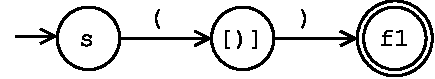
\includegraphics{fig/finiteAutomat2.pdf}
  \end{figure}

  Tento automat bude fungovat bez problému pro řetězec \symb{()},
  my ale chceme zpracovávat i zanořené závorky a na to tento automat zatím nestačí.
  Pokud tedy chceme univerzálnější automat, stačí přidat další stav:

  \begin{figure}[H]
    \centering
    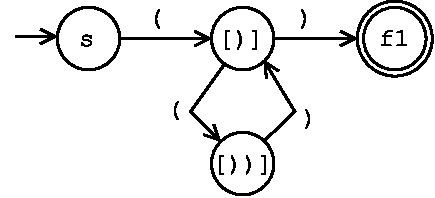
\includegraphics{fig/finiteAutomat2_1.pdf}
  \end{figure}

  Zde již zvládneme i závorky s jedním zanořením. Problémem ovšem je, že
  pro každé nové zanoření musíme přidat nový stav.
  Kdybychom tedy chtěli zpracovávat jakýkoliv počet zanoření (tedy potenciálně $\infty$),
  musel by automat obsahovat nekonečné množství stavů.
  Problémem \term{konečného automatu} je, že může obsahovat pouze konečný
  počet stavů, jelikož každý musíme nejprve definovat.
  Zde tedy vidíme příklad jazyka, který nejde zpracovávat Konečným automatem
  a z toho vyplívá, že není ani Regulárním jazykem.
  Řekněme si rovnou, že bezkontextové jazyky tento problém řeší a k tomuto
  příkladu se ještě vrátíme.

\end{exmp}

\section{Bezkontextové jazyky}

Bezkontextový jazyk je obvykle definován Bezkontextovou gramatikou.
Jak jsme již uvedli v \term{Chomského hierarchii} (str. \pageref{subsec:chomHierarchy}),
tyto gramatiky obsahují pravidla ve tvaru $A \rightarrow \gamma$, kde $A$ je neterminál a
$\gamma$ řetězec terminálů a neterminálů.

\subsection{Bezkontextové gramatiky}
\label{subsec:contextFreeGrammars}
Pokračujme nyní v příkladu \ref{exmp:brackets} a ukažme si, jak ho lze
vyjádřit pomocí bezkontextové gramatiky.\\

Chceme tedy vyjádřit výraz tvořený závorkami, pomocí gramatických pravidel.
Označme dvojici závorek jako výraz = neterminál $E$. Gramatické pravidlo tedy bude
vypadat takto:
\[E \rightarrow ()\]
Nyní bychom ale chtěli vyjádřit, že uvnitř závorek může být další výraz, to
lze udělat tímto rekurzivním způsobem:
\[E \rightarrow (E)\]
Zkusme nyní rozgenerovávat výraz E, tak jak to bylo naznačeno na Obr. \ref{img:rewriteRule},
tedy pomocí přepisování neterminálů:
\begin{lstlisting}
  1.        E
  2.       (E)
  3.      ((E))
  4.     (((E)))
  5.       ...
\end{lstlisting}
Vidíme, že zanořování, které nám dělalo problémy u regulárních jazyků, zde vyjádříme bez problému,
ještě by to však chtělo několik vylepšení.
Můžeme si všimnout, že rozgenerovávání by se vlastně mělo provádět do nekonečna,
protože neterminálu E se nyní nelze zbavit. To lze vyřešit přidáním tzv.
$\varepsilon$-pravidla:
\[E \rightarrow \varepsilon\]
To nám říká, že neterminál E je možno kdykoliv vymazat. Dále bychom ještě chtěli,
aby se za závorkou mohla vyskytovat další závorka, např. \symb{(()())}.
Stačí přidat do výrazu další rekurzi:
\[E \rightarrow (E)E\]
Všimněme si ještě, že začínáme od symbolu $E$, který lze vymazat pomocí
$\varepsilon$-pravidla, přijímáme tedy i prázdný řetězec. Pokud bychom chtěli
vyjádřit, že celý výraz musí být alespoň v jedněch závrokách lze to udělat
přidáním speciálního počátečního pravidla:
\[S \rightarrow (E)\]
Nyní tedy budeme začínat od symbolu S. Označme si tuto gramatiku jako
$G$ a vyjádřeme ji formálně:

\begin{lstlisting}
  G = (
    {S, E},           (* // množina neterminálů *)
    {(, )},           (* // množina terminálů *)
    {                 (* // množina pravidel *)
      S $\rightarrow$ (E),
      E $\rightarrow$ (E)E,
      E $\rightarrow$ $\varepsilon$
    },
    S                 (* // počáteční symbol *)
  )
\end{lstlisting}

Je zřejmé, že bezkontextovými jazyky jsme schopni popsat mnohem
složitější jazyky, než regulárními jazyky. Daní za větší \term{vyjadřovací sílu}
je ale znatelně složitější zpracování těchto jazyků.

\subsection{Derivační strom}
\label{subsec:derivationTree}
Při aplikaci gramatiky na řetězec jde vlastně o ověření,
jestli lze z počátečního symbolu,
postupnou derivací (aplikací pravidel gramatiky) získat daný řetězec.
Mějme například gramatiku:

\begin{lstlisting}
  G = (
    {E},
    {*, +, a},
    {
      E $\rightarrow$ E*E,
      E $\rightarrow$ E+E,
      E $\rightarrow$ a
    },
    E
  )
\end{lstlisting}
\noindent
Pravidla této gramatiky lze vyjádřit pomocí elementárního stromu,
kde levá strana je kořen a pravá strana představuje jeho potomky.
Např. první pravidlo z gramatiky $G$ lze znázornit stromem takto:
\begin{figure}[H]
  \centering
  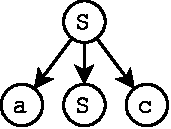
\includegraphics{fig/RuleTree1.pdf}
\end{figure}

\noindent
Pro menší velikost grafu budeme ale pravidla zjednodušeně znázorňovat takto:

\begin{figure}[H]
  \centering
  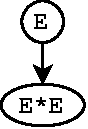
\includegraphics{fig/RuleTree2.pdf}
\end{figure}

\noindent
Pro příklad postupné derivace mějme řetězec $s$:

\begin{lstlisting}
  a * a + a
\end{lstlisting}

\noindent
Nyní zkusíme postupně aplikovat pravidla na počáteční symbol,
tak abychom získali řetězec $s$
(v komentáři jsou uvedena pravidla, která byla použita):

\begin{lstlisting}
   E
  E*E                   // E $\rightarrow$ E*E(*\footnote{Zde bychom mohli použít
    i pravidlo $E \rightarrow E + E$ a dostali bychom odlišný strom (viz. Sekce \ref{subec:nondeterminsm})}*)
  a*E                   // E $\rightarrow$ a
  a*E+E                 // E $\rightarrow$ E+E
  a*a+E                 // E $\rightarrow$ a
  a*a+a                 // E $\rightarrow$ a
\end{lstlisting}

\noindent
Touto posloupností derivací jsme byli schopni dosáhnout kontrolovaného řetězce $s$,
daný řetězec tedy patří do gramatiky. Výše zobrazené derivace lze zobrazit
i jinak a to pomocí tzv. \term{Derivačního stromu}:

\begin{figure}[H]
  \centering
  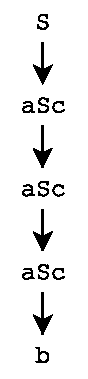
\includegraphics{fig/Derivations1.pdf}
\end{figure}

\noindent
Pro větší názornost ukažme ještě stejný strom s přiřazenými symboly k původnímu
řetězci a vyznačenými jednotlivými úrovněmi.

\begin{figure}[H]
  \centering
  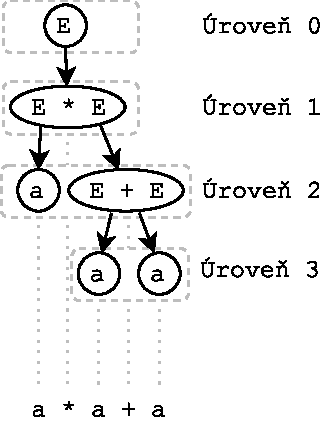
\includegraphics{fig/Derivations2.pdf}
\end{figure}

\begin{defn}
  (Derivační strom). \cite[str. 92]{MedunaIFJ}\\
  Nechť $G = (\Sigma, R)$ je Bezkontextová gramatika.\\
  \begin{enumerate}
    \item Pro $l$: $A \rightarrow x \in R, A\langle x\rangle$ je strom pravidla, které reprezentuje $l$.
    \item Derivační strom reprezentující derivace v $G$ je definován rekurzivně:
    \begin{enumerate}
      \item Strom s jedním uzlem $X$ je derivační strom odpovídající $X \Rightarrow^0 X$ v $G$, kde $X \in \Sigma$.
      \item Nechť $d$ je derivační strom reprezentující
            $A \Rightarrow^0 uBv$ [$\rho$] s hranicí($d$) $ = uBv$, a nechť $l: B \rightarrow z \in R$.
            Derivační strom, který reprezentuje
            \begin{align}
                A & \Rightarrow^* uBv [\rho] \nonumber\\
                  & \Rightarrow \hphantom{*} uzv [l] \nonumber
            \end{align}
            je získán nahrazením ($|u|+1$)-tého listu v $d$, $B$, stromem pravidla odpovídajícho $l$, $B\langle z\rangle$
    \end{enumerate}
    \item Derivační strom v $G$ je jakékoliv $t$, pro které existuje derivace odpovídající $t$ (viz 2.).
  \end{enumerate}
  \vspace{-0.2cm}
\end{defn}

\subsection{Nedeterminismus}
\label{subec:nondeterminsm}

U příkladu z minulé sekce (\ref{subsec:derivationTree}) si můžeme všimnout,
že při konstrukci derivačního stromu máme pro jeden řetězec možnost sestrojit
2 stromy:

\begin{figure}[H]
  \centering
  \includegraphics{fig/TwoDerivationTrees.pdf}
\end{figure}

Vidíme, že generovaný řetězec je stejný, ale stromy jsou odlišné.
Takováto gramatika je označována jako nedeterministická a způsobuje problémy při
zpracování, protože v rozhodné chvíli nevíme, které pravidlo použít.\\

Protože determinismus je při implementaci zásadní, rozdělujeme Bezkontextové gramatiky
na deterministické a nedeterministické (podobně i zásobníkové automaty).\\


\subsection{Zásobníkové automaty}

Zásobníkový automat rozšiřuje \term{Konečný automat} o zásobník, kam lze
ukládat symboly (terminály i neterminály).\\

Pro rozhodnutí, jaké pravidlo použít,
využívá vedle vstupního symbolu a stavu i symbol na vrcholu zásobníku. V rámci vykonání
přechodu lze zároveň manipulovat se zásobníkem.\\

Vraťme se opět k příkladu \ref{exmp:brackets} a všiměme si stavů
vyjadřujících zanoření. Značili jsme je jako počet uzavíracích závorek,
které jsou ještě potřeba, aby byl výraz platný. Pokud jsme narazili na
otevírací závorku, přešli jsme do stavu \uv{o jedna více závorek}, v případě uzavírací
do \uv{o jedna méně závorek}. Přechody mezi stavy jsou znázorněny na
následujícím jednoduchém řetězci:

\begin{figure}[H]
  \centering
  \includegraphics{fig/bracketsAutomat.pdf}
\end{figure}

Přidávání a odebírání závorek nám může připomínat zásobník.
Zásobníkový automat dokáže tyto stavy vyjádřit zásobníkem a potom
není nutné všechny tyto stavy definovat.\\

\begin{defn}
  (Zásobníkový automat)\\
  Zásobníkový automat je sedmice $M = (Q, \Sigma, \Gamma, R, q_0, Z_0, F)$, kde:
  \begin{itemize}
    \item $Q$ je konečná množina stavů
    \item $\Sigma$ je vstupní abeceda
    \item $\Gamma$ je konečná abeceda zásobníku
    \item $R \subseteq (\Gamma \times Q \times (\Sigma \cup \{\varepsilon\} ))
    \times (\Gamma^* \cup Q)$ je konečná množina binárních relací (pravidel)
    \item $q_0 \in Q$ je počáteční stav
    \item $Z_0 \in \Gamma$ popisuje počáteční symboly na zásobníku
    \item $F \subseteq Q$ je množina konečných stavů
  \end{itemize}

  \noindent
  Pravidla $R$ zásobníkového automatu je ve tvaru $(q_1, a, z_1) \rightarrow (q_2, \gamma)$, kde:

  \begin{itemize}
    \item $q_1$ je výchozí stav
    \item $a$ je symbol na vstupu
    \item $z_1$ je symbol na vrcholu zásobníku
    \item $q_2$ je výstupní stav
    \item $\gamma$ je řetězec, který se má vložit na zásobník
  \end{itemize}
  \vspace{-0.5cm}
\end{defn}

Zásobníkovým automatem lze zpracovávat Deterministické bezkontextové jazyky.
V případě nedeterministických musíme nějak blíže specifikovat, který z možných
stromů chceme.\\

\section{Zpracování bezkontextových jazyků}
\label{sec:CFLanguagesProcessing}

Při zpracování bezkontextového jazyka je hlavní problematikou
sestavování konfigurace zasobníkového automatu pro danou gramatiku.
Musíme totiž gramatická (přepisovací) pravidla zanést do konfigurace
automatu tak, aby bylo vždy jasné, které použít.\\

Při návrhu syntaktického analyzátoru se vždy objeví otázka, zdali je lepší
při konstrukci derivačního stromu postupovat od kořene (shora dolů) nebo od
zkoumaného řetězce (zdola nahoru). Odpověď na tuto otázku není jednoznačná,
což je vidět i na široce používaných analyzátorech programovacích jazyků,
kdy se tato technika liší projekt od projektu.\\

V případě tohoto projektu je tomu nejinak, a proto v této části budeme rozebírat
obě alternativy, aby byly zřejmé jejich výhody i nevýhody.

\subsection{Syntaktická analýza shora dolů}

Nejpoužívanějším zástupcem této skupiny je \term{LL syntaktická analýza}, která analyzuje
vstup zleva doprava a konstruuje nejlevější derivaci. Tato syntaktická analýza
umožňuje zpracovávat pouze LL gramatiky,
které jsou podmnožinou deterministických bezkontextových gramatik.\\

Které pravidlo použít slouží \term{LL tabulka}, která nám na základě
vstupního symbolu a symbolu na zásobníku určí pravidlo, které se má použít.
Následující algoritmy slouží k její konstrukci.\\

\noindent
Množina $Empty(X)$ nám říká, jestli lze symbol $X$ odstranit:\\
\begin{algorithm}[H]
  \caption{$Empty(X)$}
  \KwIn{Gramatika $G = (N, \Sigma, P, S)$}
  \KwOut{$Empty(X)$ pro každý symbol $X \in N \cup \Sigma$ }

  \BlankLine
  \Begin{
    $Empty(a) := \emptyset$ pro každé $a \in \Sigma$\;
    \ForAll{$A \in N$}{
      \uIf{$A \rightarrow \varepsilon \in P$}{
        $Empty(A)$ := $\{\varepsilon\}$\;
      }
      \Else{
        $Empty(A)$ := $\emptyset$\;
      }
    }

    \Repeat{žádná z množin Empty nezměněna} {
      \If{$A \rightarrow X_1 X_2 ... X_n \in P$ \And   $Empty(X_i) = {\varepsilon}$
              pro všechna $i = 1, ... ,n$}{
        $Empty(A)$ := $\{\varepsilon\}$\;
      }
    }
  }
\end{algorithm}
\vspace{0.5cm}

\noindent
Množina $First(X)$ nám říká, které terminální symboly se mohou nacházet
na začátku symbolu $X$:\\
\begin{algorithm}[H]
  \caption{$First(X)$}
  \KwIn{Gramatika $G = (N, \Sigma, P, S)$}
  \KwOut{$First(X)$ pro každý symbol $X \in N \cup \Sigma$ }

  \BlankLine
  \Begin{
    $first(a) := \{a\}$\ pro každé $a \in \Sigma$\;
    $first(A) := \emptyset$ pro každé $A \in N$\;

    \Repeat{žádná z množin $First$ nezměněna} {
      \If{$A \rightarrow X_1 X_2 ... X_{k-1}X_k ... X_n \in P$}{
        $First(A)$ := $First(A) \cup First(X_1)$\;
        \If{$Empty(X_i) = \{\varepsilon\}$
            pro $i = 1, ..., k-1$ kde $k \leq n$}{
          $First(A)$ := $First(A) \cup First(X_k)$\;
        }
      }
    }
  }
\end{algorithm}
\vspace{0.5cm}

\noindent
Množina $Empty(X_1X_2 ... X_n)$ nám říká, jestli lze řetězec
$X_1X_2 ... X_n$ odstranit:\\
\begin{algorithm}[H]
  \caption{$Empty(X_1X_2 ... X_n)$}
  \KwIn{Gramatika $G = (N, \Sigma, P, S)$; $Empty(X)$
        pro každé $X \in N \cup T$; $x = X_1X_2 ... X_n$,
        kde $x \in (N \cup T)^+$}
  \KwOut{$Empty(X_1X_2 ... X_n)$}

  \BlankLine
  \Begin{
    \uIf{$Empty(X_i) = \{\varepsilon\}$ pro každé $i = 1, ..., n$}{
      $Empty(X_1X_2 ... X_n)$ := $\{\varepsilon\}$\;
    }
    \Else{
      $Empty(X_1X_2 ... X_n)$ := $\emptyset$\;
    }
  }
\end{algorithm}
\vspace{0.5cm}

\noindent
Množina $First(X_1X_2 ... X_n)$ nám říká, které terminální symboly
se mohou nacházet na začátku řetězce $X_1X_2 ... X_n$:\\
\begin{algorithm}[H]
  \caption{$First(X_1X_2 ... X_n)$}
  \KwIn{Gramatika $G = (N, \Sigma, P, S)$; $First(X)$ a $Empty(X)$
        pro každé $X \in N \cup T$; $x = X_1X_2 ... X_n$,
        kde $x \in (N \cup T)^+$}
  \KwOut{$First(X_1X_2 ... X_n)$}

  \BlankLine
  \Begin{
    $First(X_1X_2 ... X_n)$ := $First(X_1)$\;

    \Repeat{množina $First(X_1X_2 ... X_{k-1}X_k ... X_n)$ nezměněna} {
      \If{$Empty(X_i) = \{\varepsilon\}$
          pro $i = 1, ..., k-1$ kde $k \leq n$}{
        $First(X_1X_2 ... X_n)$ := $First(X_1X_2 ... X_n) \cup First(X_k)$\;
      }
    }
  }
\end{algorithm}
\vspace{0.5cm}

\noindent
Množina $Follow(X)$ říká, které terminální symboly se mohou nacházet
za symbolem $X$:\\
\begin{algorithm}[H]
  \caption{$Follow(X)$}
  \label{alg:follow}
  \KwIn{Gramatika $G = (N, \Sigma, P, S)$}
  \KwOut{$Follow(A)$ pro každý symbol $A \in N$}

  \BlankLine
  \Begin{
    $Follow(S) := \{\$\}$\;

    \Repeat{žádná z množin $Follow$ nezměněna} {
      \If{$A \rightarrow xBy \in P$}{
        \If{$y \neq \varepsilon$}{
          $Follow(B)$ := $Follow(B) \cup First(y)$\;
        }
        \If{$Empty(y) = \{\varepsilon\}$
            pro $i = 1, ..., k-1$ kde $k \leq n$}{
          $Follow(B)$ := $Follow(B) \cup Follow(A)$\;
        }
      }
    }
  }
\end{algorithm}
\vspace{0.5cm}

\noindent
Množina $Predict(A \rightarrow x)$ říká, které terminální symboly mohou být
na vstupu pro pravidlo $A \rightarrow x$:
\begin{defn}
  (Množina $Predict(A \rightarrow x)$)\\
  Nechť $G = (N, \Sigma, P, S)$ je Bezkontextová gramatika.
  Pro každé $A \rightarrow x \in P$ definujeme množinu
  $Predict(A \rightarrow x \in P)$ takto:
  \begin{description}
    \item[Pokud $Empty(x) = \{\varepsilon\}$ potom:]\hfill \\
    $Predict(A \rightarrow x \in P) = First(x) \cup Follow(A)$
    \item[Jinak:]\hfill \\
    $Predict(A \rightarrow x \in P) = First(x)$
  \end{description}
\end{defn}
\vspace{0.5cm}

\noindent
Zbývá už jen naplnit LL tabulku pro funkci $\alpha(A, a)$, která nám pro neterminál
a terminál vrátí pravidlo, které použít:\\
\begin{algorithm}[H]
  \caption{$\alpha(A, a)$}
  \KwIn{Gramatika $G = (N, \Sigma, P, S)$; $Predict(A \rightarrow x)$, pro každé pravidlo z $P$}
  \KwOut{$\alpha(A, a)$, pro všechny platné kombinace $(A, a)$}

  \BlankLine
  \Begin{
    \ForAll{$A \rightarrow a \in P$} {
      \ForAll{$b \in Predict(A \rightarrow a)$}{
        \uIf{$\alpha(A, b)$ není definováno}{
          $\alpha(A, b) = A \rightarrow a$
        }
        \Else{
          chyba - nejde o LL gramatiku
        }
      }
    }
  }
\end{algorithm}
\vspace{0.5cm}

Chybový stav v posledním algoritmu nám vlastně indikuje nedeterminismus
v LL tabulce - tedy že pro nějakou kombinaci [$A, a$] by v LL tabulce bylo
více záznamů, takže bychom nevěděli, které pravidlo použít.\\

\noindent
Vraťme se nyní ke gramatice $G$ (z kapitoly \ref{subsec:contextFreeGrammars}):
\begin{exmp}

\begin{lstlisting}

  G = (
    {S, E},           (* // množina neterminálů *)
    {(, )},           (* // množina terminálů *)
    {                 (* // množina pravidel *)
      S $\rightarrow$ (E),         (* // pravidlo 1 *)
      E $\rightarrow$ (E)E,        (* // pravidlo 2 *)
      E $\rightarrow$ $\varepsilon$             (* // pravidlo 3 *)
    },
    S                 (* // počáteční symbol *)
  )
\end{lstlisting}
\noindent
LL tabulku bychom podle výše uvedených algoritmů sestavili takto:
\begin{table}[H]
  \centering
  \begin{tabular}{| c || c | c | c |}
    \hline
      & ( & ) & \$ \\
    \hhline{|=||=|=|=|}
    S & 1 &   &    \\
    \hline
    E & 2 & 3 &    \\
    \hline
  \end{tabular}
  \caption{LL tabulka gramatiky G s čísly pravidel}
\end{table}


Nyní zkusme zpracovat řetězec \symb{(())} gramatikou $G$
s pomocí LL tabulky.
Vlevo je znázorněný zásobník (s vrcholem)
a šipky ukazují na aktuální vstupní symbol.
Speciální znak \symb{\$} nám značí konec vstupu.

\begin{figure}[H]
  \centering
  \subfloat[Zpracování řetězce]{
    \includegraphics[scale=0.6]{fig/bracketsCFAutomat.pdf}
  }
  \subfloat[Derivační strom]{
    \hspace{1cm}
    \includegraphics{fig/bracktesDerivationTree.pdf}
    \hspace{1cm}
  }
\end{figure}

Při zpracování jsme postupovali tak jako zásobníkový automat.
Před zahájením algoritmu vložíme na zásobník symbol \symb{\$}
a počáteční symbol \symb{S}. Vysvětleme podrobně některé kroky (číslování odpovídá obrázku):

\begin{itemize}
  \item[1.] Na zásobníku je neterminál \symb{S} - na základě vstupu \symb{(} vybereme
  z LL tabulky pravidlo 1 a nahradíme S za pravou stranu pravidla
  \item[2.] Na zásobníku je terminál \symb{(} a shoduje se se vstupním symbolem - můžeme jej odstranit
  \item[3.] Na zásobníku je neterminál \symb{E} a na vstupu opět \symb{(}, použijeme pravidlo 2
  \item[4.] Na zásobníku je terminál \symb{(} a shoduje se se vstupem - odstraníme
  \item[5.] Na zásobníku je neterminál \symb{E} a na vstupu \symb{)} - použijeme pravidlo 3
  \item[] ...
  \item[9.] Na zásobníku je terminál \symb{\$} a shoduje se se vstupem - při tomto znaku skončíme
\end{itemize}
\end{exmp}

\noindent
Při zpracování mohou nastat následující chyby:

\begin{itemize}
  \item Znak na vstupu není v abecedě
  \item V LL tabulce není pravidlo pro danou kombinaci neterminálu a terminálu
  \item Terminály na vstupu a vrcholu zásobníku se neschodují
\end{itemize}

\noindent
Všechny tyto případy znamenají, že řetězec nepatří do gramatiky $G$

\subsection{Syntaktická analýza zdola nahoru}

Syntaktická analýza zdola nahoru sestavuje derivační strom odspodu,
tedy začíná neterminály a postupně se propracuje až k počátečnímu symbolu
gramatiky.


\subsubsection*{LR syntaktická analýza}
Pro účely této práce se budeme zabývat \term{LR syntaktickou analýzou}, jelikož
parsery tohoto typu mohou mít až sílu ekvivalentní s \term{Deterministickým zásobníkovým
automatem}\cite[str. 155]{MedunaIFJ}, tedy představují nejsilnější nástroj
v oblasti \term{Deterministických bezkontextových jazyků}.
LR syntaktická analýza generuje obrácený pravý rozbor.\\

Pro zpracování se opět používá \term{Zásobníkový automat}, který je
rozšířen o možnost pracovat na vrcholu zásobníku s řetězecem (ne jen s jedním symbolem).
Toto rozšíření je nutné pro aplikování pravidel - tedy nahrazení řetězce na pravé straně za
symbol na levé straně pravidla (postupujeme opačně než u LL).\\

Při analýze řetězce dáváme postupně příchozí symboly na zásobník (operace \term{shift})
a v určité chvíli použijeme pravidlo a nahradíme symboly na vrcholu zásobníku za
jeho levou stranu (operace \term{reduce}). Kterou operaci v dané chvíli provést
nám určuje tzv. LR tabulka, jejíž konstrukcí se budeme dále zabývat.\\

\subsubsection*{LR tabulka}

\term{LR tabulka} je poněkud složitější, než \term{LL tabulka}. Obsahuje 2 části:

\begin{itemize}
  \item Akční část je definována jako $\alpha(q, a)$ kde $q$ je stav a $a$ je terminál.\\
  Určuje jakou operaci provést a k tomu informaci
  do jakého stavu přejít (u op. shift) nebo jaké pravidlo použít (op. reduce), a také speciální
  ukončovací symbol
  \item Přechodová část je definována jako $\beta(q, A)$ kde $q$ je stav a $A$ je neterminál.\\
  Určuje do jakého stavu přejít po aplikaci pravidla.
\end{itemize}

Stav zde vyjadřuje možnosti, které vyplívají ze znaků naposledy přečtených.
Pro každý stav existuje množina pravidel, jejichž pravá strana prozatím vyhovuje přečteným symbolům.
Při znázorňování množin pravidel budeme používat znak \symb{•} znázorňující aktuální pozici v pravidle.\\

\noindent
Algoritmus $Closure(I)$ je definován pro pravidlo s určenou pozicí a generuje z něj stavovou skupinu:\\
\begin{algorithm}[H]
  \caption{$Closure(I)$}
  \KwIn{Gramatika $G = (N, \Sigma, P, S)$; Položka $I$}
  \KwOut{$Closure(I)$}

  \BlankLine
  \Begin{
    $Closure(I)$ := $\{I\}$\;
    \Repeat{množina $Closure(I)$ nezměněna}{
      \If{$A \rightarrow y$•$Bz \in Closure(I)$ \And $B \rightarrow x \in P$} {
        $Closure(I)$ := $Closure(I) \cup B \rightarrow $ •$x$\;
      }
    }
  }
\end{algorithm}
\vspace{0.5cm}

\noindent
Následující algoritmus vytvoří množinu $\Theta_G$ všech stavových množin pro gramatiku $G$ rozšířenou o
pravidlo $S' \rightarrow S$, kde $S$ je počáteční symbol:\\
\begin{algorithm}[H]
  \caption{$\Theta_G$}
  \label{alg:groups}
  \KwIn{Rozšířená gramatika $G = (N, \Sigma, P, S')$}
  \KwOut{$\Theta_G$}

  \BlankLine
  \Begin{
    $\Theta_G$ := $\{Closure(S' \rightarrow $ •$S)\}$\;
    \ForAll{$I \in \Theta_G$ \And $U \in N \cup \Sigma$}{
      \If{$\Theta_U(I) \neq \emptyset$} {
        přidej $\Theta_U(I)$ do $\Theta_G$;
      }
    }
  }
\end{algorithm}
\vspace{0.5cm}

\noindent
Nyní sestrojíme LR tabulku, pomocí SLR algoritmu. Budeme zde potřebovat také
algoritmus \ref{alg:follow} ($Follow$). Operaci shift znázorňujeme jako $s$,
reduce jako $r$. Ukončovací symbol označme jako a (accept).\\
\begin{algorithm}[H]
  \caption{$SLR$}
  \KwIn{Rozšířená gramatika $G = (N, \Sigma, P, S')$;
    $\Theta_G;$ $Follow(A)$ pro všechna $A \in N$}
  \KwOut{LR tabulka pro $G$ ($\alpha$ = akční č., $\beta$ = přechodová č.)}

  \BlankLine
  \Begin{
    \ForAll{$x \in \Theta_G$}{
      \ForAll{$I \in x$}{
        \Switch{$I$}{
          \Case{$I = A \rightarrow y$•$Xz$, kde $X \in N$:}{
            $\beta[x, X] := \Theta_X(x)$ \tcp*{$\beta$ část}
          }
          \Case{$I = A \rightarrow y$•$Xz$, kde $X \in \Sigma$:}{
            $\alpha[x, X] := s\Theta_X(x)$ \tcp*{operace shift}
          }
          \Case{$I = S' \rightarrow S$•:}{
            $\alpha[x, \$]$ := a  \tcp*{úspěšný konec}
          }
          \Case{$A \rightarrow y$• $(A \neq S')$:}{
            \ForAll{$a \in Follow(A)$}{
              $\alpha[x, a]$ := $rp$,
              kde $p$ je číslo pravidla $A \rightarrow y$ \tcp*{reduce}
            }
          }
        }
      }
    }
  }
\end{algorithm}
\vspace{0.5cm}

\noindent
Syntaktická analýza využívající LR tabulku vypadá takto:\\
\begin{algorithm}[H]
  \caption{LR syntaktická analýza}
  \label{alg:lr}
  \KwIn{LR tabulka pro $G = (N, \Sigma, P, S)$ a řetězec $x \in T^*$}
  \KwOut{Pravý rozbor $x$, pokud $x \in L(G)$, jinak chyba}

  \BlankLine
  \Begin{
    Vlož $\langle\$,q_0\rangle$ na zásobník\;
    $stav$ := $q_0$\;
    \Repeat{úspěch \Or chyba}{
      $a$ = aktuální znak na vstupu\;
      \Switch{$\alpha[stav, a]$}{
        \uCase{$sq$:}{
          push($\langle a, q\rangle$)\;
          přečti další znak $a$ ze vstupu\;
          stav := q\;
        }
        \uCase{$rp$}{
          \uIf{$p$: $A \rightarrow X_1X_2 ... X_n \in P$ \And
            $\langle?,q\rangle\langle X_1, ?\rangle\langle X_2, ?\rangle ... \langle X_n, ?\rangle$
              je na vrcholu zásobníku}{
            $stav$ := $\beta[q,A]$\;
            zaměň na zásobníku $\langle X_1, ?\rangle\langle X_2, ?\rangle ... \langle X_n, ?\rangle$
              za $\langle A, stav\rangle$\;
            zapiš $p$ na výstup\;
          }
          \Else{
            chyba
          }
        }
        \uCase{a}{
          úspěch
        }
        \Case{nedefinováno}{
          chyba
        }
      }
    }
  }
\end{algorithm}
\vspace{0.5cm}

\begin{exmp} Vezměme gramatiku $G$ z kapitoly \ref{subsec:derivationTree}:


\begin{lstlisting}
  G = (
    {E},
    {*, +, a},
    {
      S' $\rightarrow$ E,               // pravidlo 0 (*(přidané)*)
      E $\rightarrow$ E*E,              // pravidlo 1
      E $\rightarrow$ E+E,              // pravidlo 2
      E $\rightarrow$ a                 // pravidlo 3
    },
    E
  )
\end{lstlisting}

\noindent
Stavové skupiny $\Theta_G$ z algoritmu \ref{alg:groups} pro tuto gramatiku vypadají takto:
\begin{lstlisting}
  0: S' -> (*•*)E, E -> (*•*)E*E, E -> (*•*)E+E, E -> (*•*)a
  1: S' -> E(*•*), E -> E(*•*)*E, E -> E(*•*)+E
  2: E -> a(*•*)
  3: E -> E*(*•*)E, E -> (*•*)E*E, E -> (*•*)E+E, E -> (*•*)a
  4: E -> E+(*•*)E, E -> (*•*)E*E, E -> (*•*)E+E, E -> (*•*)a
  5: E -> E*E(*•*), E -> E(*•*)*E, E -> E(*•*)+E
  6: E -> E+E(*•*), E -> E(*•*)*E, E -> E(*•*)+E
\end{lstlisting}

\noindent
Zde je LR tabulka:

\begin{table}[H]
  \catcode`\-=12
  \centering
  \begin{tabular}{| c || c | c | c | c || c | c |}
    \hline
    \multirow{2}{*}{} & \multicolumn{4}{c||}{$\alpha$}& \multicolumn{2}{c|}{$\beta$} \\
    \cline{2-7}
      & * & + & a & \$& S'& E \\
    \hhline{|=||=|=|=|=||=|=|}
    0 &   &   & s1 &   &   & 2 \\
    \hline
    1 & r3 & r3 &   & r3 &   &   \\
    \hline
    2 & s3 & s4 &   & a &   &   \\
    \hline
    3 &   &   & s1 &   &   & 5 \\
    \hline
    4 &   &   & s1 &   &   & 6 \\
    \hline
    5 & s3 r1 &  s4 r1 & & r1 &   & \\
    \hline
    6 & s3 r2 &  s4 r2 & & r2 &   & \\
    \hline
  \end{tabular}
\end{table}

Všimněme si, že v některých polích tabulky máme 2 položky. Tyto případy
se nazývají \term{shift-reduce} konflikty a jsou projevem toho, že je tato
gramatika nedeterministická (viz. sekce \ref{subec:nondeterminsm}).
Výhodou LR gramatiky je to, že ji lze lehce rozšířit o priority operátorů
a poté za běhu rozhodnout, které pravidlo použít.
Priority pro tuto gramatiku mohou vypadat následovně:

\begin{lstlisting}
  left: *
  left: +
\end{lstlisting}

V tomto případě má tedy operátor  \symb{*} vyšší prioritu a oba operátory jsou vyhodnocovány zleva.
Za běhu poté porovnáváme příchozí neterminál s posledním operátorem na zásobníku
a na základě toho rozhodneme jestli provedeme operaci \term{shift} nebo \term{reduce}.
Ukažme si zpracování řetězce \symb{a * a + a}:

\begin{figure}[H]
  \centering
  \subfloat[Zpracování řetězce]{
    \includegraphics[scale=0.6]{fig/exprLRParsing.pdf}
  }
  \subfloat[Derivační strom]{
    \hspace{1cm}
    \includegraphics{fig/exprDerivationTree.pdf}
    \hspace{1cm}
  }
\end{figure}

Ve výše zobrazeném diagramu postupujeme podle algoritmu \ref{alg:lr},
vysvětleme některé kroky:
\begin{itemize}
  \item[1.] Jsme ve stavu 0 a na vstupu máme \symb{a} - podle LR tabulky přejdeme do
  stavu 1 a provedeme operaci \term{shift} (vložíme \symb{a} na zásobník s aktuálním stavem).
  \item[2.] Jsme ve stavu 1 a na vstupu máme \symb{*} - podle LR tabulky provedeme
  operaci \term{reduce} podle pravidla 3 - poslední stav za nahrazovanou částí na
  zásobníku je 0 a levá strana pravidla je \symb{E} - podle beta části LR tabulky
  přejdeme do stavu 2 (vložíme na zásobník i s neterminálem \symb{E}).
  \item[3.] Jsme ve stavu 2 a na vstupu máme \symb{*} - \term{shift} 3.
  \item[4.] Jsme ve stavu 3 a na vstupu máme \symb{a} - \term{shift} 1.
  \item[5.] Jsme ve stavu 1 a na vstupu máme \symb{+} - \term{reduce} 3
   - poslední stav je 3 a levá strana je \symb{E} - přejdeme do stavu 5.
  \item[6.] Jsme ve stavu 5 a na vstupu máme \symb{+} - narazili jsme na \term{shift-reduce} konflikt
  v LR tabulce - poslední operátor na zásobníku je \symb{*}, protože má vyšší prioritu,
  provedeme operaci \term{reduce} 1 - poslední stav je 0 a levá strana je \symb{E} - přejdeme do stavu 2.
  \item[] ...
  \item[11.] Jsme ve stavu 2 a na vstupu máme \symb{\$} - V LR tabulce je \symb{a}
  (Accept) - můžeme skončit a řetězec prohlásit za přijatý.
\end{itemize}
\end{exmp}

Je vidět, že pomocí LR syntatické analýzy jsme schopni zpracovávat deterministické
gramatiky a pokud přidáme priority, i některé nedeterministické. Všimněme si jak je
sestavován derivační strom - jdeme odspodu a vytváříme několik podstromů,
teprve v posledním kroku je spojíme do jednoho.


\chapter{Zpracování jazyků řízených stromy}
\label{ch:processingTreeLanguages}

Pro dosažení větší síly syntaktického analyzátoru bývají zásobníkové automaty
rozšiřovány o další funkce (tím se odchylují od původního matematického modelu).
Příkladem takové techniky může být již uvedená \term{priorita operátorů}.
V této kapitole se budeme zabývat jazyky řízenými stromy a rozšířením
zásobníkového automatu, aby byl schopen takové jazyky zpracovávat.\\

\section{Omezení úrovní derivačního stromu}

Ve své práci jsem se rozhodl pro techinku omezování derivačního stromu pomocí
kontroly jeho úrovní regulárním jazykem.
Gramatika jazyka řízeného stromem se tedy skládá ze 2 částí a značíme ji jako
$(G, R)$, kde:
\begin{itemize}
  \item $G$ je bezkontextová \term{řídicí gramatika}, slouží ke konstrukci derivačního stromu
  pro daný řetězec
  \item $R$ je \term{kontrolní jazyk} (budeme využívat regulární jazyk),
  slouží pro kontrolu úrovní derivačního stromu
\end{itemize}

\noindent
Vyjádřeno formálně:

\begin{defn}
  (Gramatiky řízené stromy)\\
  Gramatika řízená stromem je dvojice $(G, R)$, kde $G = (V, T, P, S)$
  je \term{řídicí gramatika} a $R \subseteq V^*$ \term{kontrolní jazyk}.
\end{defn}

\begin{defn}
  \label{defn:treeControlledLanguages}
  (Jazyky řízené stromy)\\
  Nechť $(G, R)$ je gramatika řízená stromem.
  Jazyk generovaný $(G, R)$ je značen jako $L(G, R)$ a definován jako:
  \vspace{5pt}
  \begin{adjustwidth}{0.5cm}{0.5cm}
    $L(G, R) = \{x: x \in L(G, R)$ a existuje derivační strom $t$ pro
    každé $x$ v $G$ takový, že každé slovo získané konkatenací
    všech symbolů na kterékoliv úrovni $t$ (kromě poslení) zleva doprava,
    patří do $R \}$.
  \end{adjustwidth}
\end{defn}

\noindent
Takto specifikovaný jazyk má vyjadřovací sílu Rekurzivně vyčíslitelných jazyků.\cite{Koutny}
Ukážeme si ovšem, že pokud se pokusíme sestrojit analyzátor takového jazyka
narazíme na řadu potíží, které výslednou vyjadřovací sílu citelně sníží.

Pro lepší porozumění následuje podrobný praktický příklad, jak lze
ověřovat příslušnost řetězce do dané gramatiky řízené stromem.

\begin{exmp}
  \label{exmp:abc}
  Mějme stromem řízený jazyk $L(G, R)$, kde:
  \begin{lstlisting}
  G = (
    {S, A, B, C, a, b, c},
    {a, b, c},
    {
      S $\rightarrow$ ABC,
      A $\rightarrow$ aA,
      A $\rightarrow$ a,
      B $\rightarrow$ bB,
      B $\rightarrow$ b,
      C $\rightarrow$ cC,
      C $\rightarrow$ c
    },
    S
  ),
  R = {S, ABC, aAbBcC}
  \end{lstlisting}
  \noindent
  A řetězec:

  \begin{lstlisting}
  aabbcc
  \end{lstlisting}

  \noindent
  Nejprve sestavíme derivační strom pro daný řetězec, poté projdeme všechny
  jeho úrovně (kromě poslední, viz. Definice \ref{defn:treeControlledLanguages}) a
  ověříme, že patří do kontrolního jazyka $R$.

  \begin{figure}[H]
    \centering
    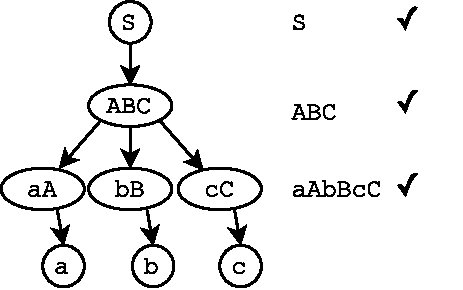
\includegraphics{fig/TreeControlledGrammar1.pdf}
  \end{figure}

  \noindent
  Z grafu je zřejmé, že v tomto případě řetězec patří do jazyka $L$.
  Zkusme však ještě jiný případ pro tento řetězec:

  \begin{lstlisting}
  aabcc
  \end{lstlisting}

  \noindent
  A jemu odpovídající derivační strom:
  \begin{figure}[H]
    \centering
    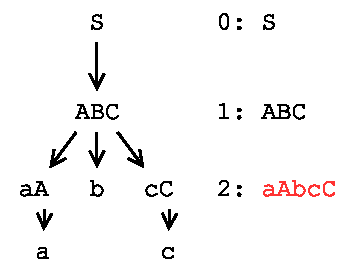
\includegraphics{fig/TreeControlledGrammar2.pdf}
  \end{figure}

  \noindent
  V tomto případě úroveň 2 derivačního stromu nepatří do kontrolního jazyka $R$,
  proto tento řetězec nepatří do jazyka $L$.
\end{exmp}

Ukázali jsme si, že samotná kontrola úrovní derivačního stromu není nijak
velkým problémem. Potřebujeme však nejdříve derivační strom zkonstruovat,
na což se zaměříme v další sekci.

\section{Sestavení derivačního stromu}

Zásadním problémem při konstrukci derivačního stromu je nedeterminismus,
který vede k tomu, že máme pro jeden řetězec více derivačních stromů.
Jelikož kontrola úrovní stromu rozhoduje o příslušnosti řetězce do jazyka,
mohlo by se stát, že některé derivační stromy by kontrolou prošly a jiné ne.
V tomto případě bychom museli sestrojit všechny derivační stromy a poté
u všech zkontrolovat úrovně. Nedeterministické analyzátory jsou ovšem řádově
pomalejší, než deterministické, proto se držme těch deterministických a
zkusme prozkoumat jinou možnost a tou je kontrolovat úrovně již při konstrukci
derivačního stromu.\\

Projděme nyní znovu 2 hlavní metody pro syntaktickou analýzu bezkontextových
deterministických jazyků (rozebírané v sekci \ref{sec:CFLanguagesProcessing})
z praktického pohledu a zamysleme se nad tím, jak by se daly k tomuto účelu
využít.

\subsection{LL syntaktická analýza}

Výhodou LL analýzy je intuitivní konstrukce derivačního stromu shora a zleva,
při tomto postupu je výhodné, že vždy máme nejlevěší část stromu, pokud tedy
chceme kontrolovat úrovně již za běhu, můžeme to provádět bez problému, jelikož
každou úroveň generujeme od nejlevějšího znaku a můžeme ji tedy rovnou
kontrolovat automatem.\\

\noindent
Na následujícím příkladu si ukažme postup při kontrole derivačního stromu:
\begin{exmp}
  \label{exmp:WW}
  \begin{lstlisting}

  G = (
    {S, W},
    {0, 1, #},
    {
      S $\rightarrow$ W#W,
      W $\rightarrow$ 0W,
      W $\rightarrow$ 1W,
      W $\rightarrow$ $\varepsilon$
    },
    S
  ),
  R = {S, W#W, 0W0W, 1W1W}
  \end{lstlisting}

  \noindent
  Pro řetězec \symb{01\#11}, vypadá LL konstrukce derivačního stromu takto:

  \begin{figure}[H]
    \centering
    \includegraphics{fig/LLTree.pdf}
  \end{figure}

  Díky tomu, že je strom generován shora a zleva můžeme jednoduše
  kontrolovat úrovně ještě před dokončením stromu. Umožňuje nám to brzké
  odhalení konfliktů v úrovni derivačního stromu, tedy zjištění, že řetězec
  nepatří do gramatiky.\\

\end{exmp}

Menší komplikaci přináší to, že z definice nekontrolujeme
nejspodnější úroveň stromu, protože u nekompletního stromu nejsme schopni určit,
jestli je daná úroveň poslední.\\
Spodní úroveň stromu však může obsahovat pouze terminály a naopak
ostatní úrovně vždy obsahují nějaký neterminál. Proto můžeme do automatu
jednoduše přidat stavy přijímající jakoukoliv posloupnost terminálů a
zkontrolovat úrovně všechny. Tato technika bude dále využívána (i u LR SA).\\

Nyní zkusme prozkoumat, jak bychom mohli těchto vlastností využít, pro
vyřešní konfliktů v ll tabulce. Ukažme si to na následující gramatice:
\begin{exmp}
  \label{exmp:aa}
  \begin{lstlisting}

  T = (G, R),
  G = (
    {S},
    {a},
    {
      S $\rightarrow$ SS,           // pravidlo 1
      S $\rightarrow$ a             // pravidlo 2
    },
    S
  ),
  R = {S$^*$}
  \end{lstlisting}
  Gramatika $T$ přijímá řetězec $a^{2^n}$. Důležité je, že
  \term{řídicí gramatika} $G$ je
  nedeterministická. Např. pro řetězec \symb{a a a a} můžeme sestrojit
  tyto stromy:

  \begin{figure}[H]
    \centering
    \includegraphics{fig/LLNondeterministic.pdf}
  \end{figure}
  Kontrolou úrovní zjistíme, že nám vyhovuje pouze strom č. 3 - z tohoto
  poznatku plyne, že pokud sestrojíme špatný strom, dojdeme k mylnému závěru
  - že řetězec nepatří do gramatiky. Má to však i velmi pozitivní důsledek:
  protože nám vyhovuje jen jeden strom celkově je gramatika $T$ vlastně
  deterministická. Dostatečně dobrá průběžná kontrola úrovní by tedy teoreticky
  měla vést pouze k jednomu správnému derivačnímu stromu.

  LL tabulka s konfliktem vypadá takto:
  \begin{table}[H]
    \centering
    \begin{tabular}{| c || c | c |}
      \hline
        & a & \$  \\
      \hhline{|=||=|=|}
      S & 0, 1 &  \\
      \hline
    \end{tabular}
  \end{table}

  Když zkusíme řetězec zpracovávat, už u prvního pravidla narazíme na zádrhel.

  \begin{figure}[H]
    \centering
    \includegraphics{fig/LLTreeConflict.pdf}
  \end{figure}

  Problémem je, že oba stromy vyhovují kontrole úrovní.
  Nejsme tedy schopni rozhodnout, který vyloučit.\\

  Mohli bychom také jednoduše zkusit jedno z pravidel a pokud bychom narazili na
  konflikt, tak se vrátit a zkusit druhé. To je již ovšem nedeterministické
  zpracování a navíc se nám zde může neblaze projevit rekurze - např. pokud bychom
  stále aplikovali pravidlo $S \rightarrow SS$ program by stále zvětšoval strom
  a na konflikt v úrovních bychom nenarazili.\\
  V tomto případě je jasné, že LL syntaktická analýza na tento problém
  není vhodná.

\end{exmp}

Problém LL syntaktické analýzy tkví v tom, že při aplikaci pravidla máme k
dispozici pouze velmi malou část stromu vytvořeného pravidlem a je tedy velmi
pravděpodobné, že nebudeme schopni určit, jestli je pravidlo správné.\\

\subsubsection*{Závěr}

Ukázali jsme si, že výhodou LL syntaktické analýzy je možnost kontrolovat
bez problému úrovně stromu již při jeho konstrukci.
Jakmile je ale \term{řídicí gramatika} nedeterministická kontrola úrovní
nám mnoho nepomůže.
Navíc LL syntaktická analýza má již v základu menší vyjadřovací sílu, než
LR syntaktická analýza, proto se pro zpracování gramatik řízených stromy
nejeví jako přílš vhodná.

\subsection{LR syntaktická analýza}
\label{subsection:LR}
LR syntaktická analýza dokáže deterministicky zpracovávat více jazyků
než LL a nabízí také jednoduché rozšíření o prioritu operátorů,
kontrola derivačního stromu za běhu je zde však mnohem složitější,
jelikož strom vytváříme zdola. Ukažme si, jak se strom vytváří pro
gramatiku z příkladu \ref{exmp:WW} a opět řetězec \symb{01\#11}:

\begin{figure}[H]
  \centering
  \includegraphics[scale=1]{fig/LRTree1.pdf}
\end{figure}

\begin{figure}[H]
  \centering
  \includegraphics[scale=1]{fig/LRTree2.pdf}
\end{figure}

LR gramatika vytváří podstromy, které postupně spojuje do jednoho.
Pokud chceme kontrolovat úrovně za běhu, lze to jednoduše provádět pouze
u nejlevějšího aktuálního podstromu.
Vidíme, že tímto způsobem odhalíme chybu v úrovních až v posledním kroku (12).\\

\subsubsection{Zpracování nedeterministické řídicí gramatiky}

\begin{exmp}
  Vezměme gramatiku z příkladu \ref{exmp:aa}. LR tabulka pro tuto gramatiku
  vypadá takto:
  \begin{table}[H]
    \centering
    \begin{tabular}{| c || c | c | c |}
      \hline
        &	a  &	\$ &	A \\
      \hhline{|=||=|=|=|}
      0 &	s2 &    & 1 \\
      \hline
      1	& s2 & a	& 3 \\
      \hline
      2	& r2 & r2 &   \\
      \hline
      3 & s2, r1& r1 & 3 \\
      \hline
    \end{tabular}
  \end{table}

  Vidíme, že tabulce je jen jediný konflikt. Při zpracování řetězce
  \symb{aaaa} na něj poprvé narazíme, když máme následující 2 stromy:

  \begin{figure}[H]
    \centering
    \includegraphics[scale=1]{fig/LRConflict.pdf}
  \end{figure}

  Jde tedy o to, jestli stromy spojit pravidlem $1: S \rightarrow SS$, nebo přejít
  na další symbol. V tomto případě chceme stromy spojit, mohli bychom tedy
  nastavit priority tak, aby se v případě symbolů \symb{[S, a]} provedla operace
  reduce, tedy že \symb{S} má větší prioritu, než \symb{a}. Při dalším konfliktu nastane
  tato situace:

  \begin{figure}[H]
    \centering
    \includegraphics[scale=1]{fig/LRConflict2.pdf}
  \end{figure}

  Zde ovšem s prioritami pohoříme, jelikož symboly jsou stejné \symb{[S, a]},
  ovšem potřebujeme, aby se provedla operace \term{shift}. Pomocí priorit lze
  sestrojit tyto 2 stromy (podle nastavení):

  \begin{figure}[H]
    \centering
    \includegraphics[scale=1]{fig/LLConflictPriority.pdf}
  \end{figure}

  Z těchto stromů však ani jeden není ten správný. Pomocí priorit tento problém
  nevyřešíme.\\

  Zkusme podobně jako u LL syntaktické analýzy řešit konflikty v LR tabulce
  pomocí kotroly úrovní stromu. U LR SA to bude ověření, jestli lze
  dané stromy spojit (aplikovat pravidlo). Ukažme si to na předchozích
  konfliktech:

  \begin{figure}[H]
    \centering
    \includegraphics[scale=1]{fig/LRConflictLevel1.pdf}
  \end{figure}

  V tomto případě úrovně sedí, takže pravidlo použijeme.
  Další konflikt je následující:

  \begin{figure}[H]
    \centering
    \includegraphics[scale=1]{fig/LRConflictLevel2.pdf}
  \end{figure}

  Zde nám již kontrola úrovní neprojde, takže provedeme shift.
  Další konflikt už nenastane a výsledný strom vypadá takto:

  \begin{figure}[H]
    \centering
    \includegraphics[scale=1]{fig/LRConflictLevel3.pdf}
  \end{figure}

  Sestrojili jsme jediný správný strom, který vyhovuje kontrole úrovní.
\end{exmp}

Vraťme se ještě ke kroku, kdy se rozhodujeme mezi operacemi \term{shift} a
\term{reduce} podle kontroly úrovní. V tu chvíli vlastně zkusíme provést
\term{reduce} a pokud dojde ke konfliktu v úrovních, provedeme \term{shift}.
Bohužel nejsme schopni určit, jestli operace \term{shift} povede ke konfliktu,
proto v případě, že pokus o \term{reduce} projde, nezbývá než předpokládat, že
\term{shift} je tou špatnou cestou.
To ovšem neplatí obecně a pokud později narazíme na konflikt, může to
znamenat, že jsme sestrojili špatný strom.\\

Nechceme se ale ochudit o možnost pokusit se sestrojit správný strom
a např. u výše uvedené gramatiky problém není.
Musíme ale tyto situace rozlišovat, tedy v případech, kdy víme jistě,
že řetězec patří nebo nepatří do gramatiky, a kdy to jistě nevíme.\\

\subsection*{Průběžná kontrola úrovní všech stromů}

U výše uvedeného příkladu jsme ověřovali úrovně jen u nejlevějšího
podstromu. Protože byl řetězec krátký, nepůsobilo to problémy.
Když ovšem budeme kontrolovat delší řetězec vzniknou nám stejné konflikty
i v jiných podstromech. Je zde ale problém, že nevíme, jak budou později
tyto podstromy připojeny k levému podstromu a nejsme tudíž schopni
kontrolovat od počátečního znaku.\\

\begin{figure}[H]
  \centering
  \includegraphics[scale=1]{fig/LRTreeLongerConflict.pdf}
  \caption{Nerozpoznaný konflikt v pravém podstromě.}
\end{figure}

Abychom zajistili alespoň nějakou průběžnou kontrolu pravých podstromů,
lze ověřit, jestli řetězec vůbec může být v daném kontrolním
jazyce, tedy jestli je podřetězcem alespoň jednoho řetězce, který do kontrolního
jazyka patří.\\

V případě modelu konečného automatu (který pro kontrolu úrovní budeme používat),
lze tuto operaci provést tak, že místo jednoho stavu automatu budeme udržovat
množinu stavů (ve kterých bychom se mohli nacházet).\\

\begin{algorithm}[H]
  \caption{Podřetězec pomocí konečného automatu.}
  \label{alg:lr}
  \KwIn{Konečný automat $M = (Q, \Sigma, R, s, F)$, vstupní řetězec $a$}
  \KwOut{Úspěch nebo Chyba}

  \BlankLine
  \Begin{
      stavy := $Q$\;
      \ForAll{znak $c \in a$}{
        \ForAll{stav $q \in$ stavy}{
          \uIf{přechod $qc \rightarrow q_{new} \in R$}{
            nahraď v $q$ za $q_{new}$\;
          }
          \Else{
            odeber $q$ ze stavů\;
          }
        }
        \If{stavy $ = \emptyset$} {
          \Return Chyba\;
        }
      }
      \Return Úspěch\;
  }
\end{algorithm}
\vspace{0.5cm}

Tento systém nám sice zajistí slabší kontrolu než u nejlevějšího podstromu,
u výše uvedeného příkladu ale tento přístup zásadně pomůže:

\begin{figure}[H]
  \centering
  \includegraphics[scale=1]{fig/LRTreeLongerConflict2.pdf}
  \caption{Rozpoznaný konflikt v pravém podstromě.}
\end{figure}

Touto technikou samozřejmě nelze zpracovávat jakoukoliv gramatiku.
Obecně problém nastáva tehdy, když se o konfliktu ve stromě rozhoduje
v době, kdy se ještě neprojeví. Takový konflikt je poté sice rozpoznán,
ale nelze jej už vyřešit bez navracení.

\subsubsection*{Závěr}

LR syntaktická analýza již v základu dokáže zpracovávat větší množství
bezkontextových gramatik. Ukázali jsme si, že kontrola úrovní je zde
sice složitější, při správném přístupu však mohou přinést poměrně výrazné
rozšíření vyjadřovací síly syntaktického analyzátoru.
LR syntaktická analýza se ukazuje jako nejvhodnější pro zpracování
gramatik řízených stromy a je využita v praktické části toho projektu.

\chapter{Implementace}

\subsubsection*{Výběr programovacího jazyka}

Z čistě praktických důvodů byl pro implementaci vybrán jazyk Python
(verze 3.4). Jde o jazyk skriptovací a vysokoúrovňový, lze tedy
očekávat nižší rychlost oproti kompilovaným a nízkoúrovňovějším jazykům.
Jelikož však tato aplikace slouží převážně pro demonstrační účely,
není rychlost tím zásadním parametrem a je tedy možné využít
výhod, jež vysokoúrovňový jazyk nabízí.

\subsubsection*{Uživatelské rozhraní}

Jelikož aplikace pracuje pouze s textovým vstupem je program koncipován
jako konzolová aplikace, ovládá se tedy výhradně přes příkazový řádek.

\subsubsection*{Vstupní parametry}

Aplikace přijímá parametry ve standardním UNIXovém formátu, jejich přesný
formát je uveden v nápovědě (argument \texttt{--help}).\\

Jediným povinným argumentem je vstupní gramatika, jež je načtena z
externího souboru. Hlavní součástí tohoto souboru je řídicí bezkontextová gramatika,
volitelně poté můžeme přidat kontrolní jazyk
(ve formě výčtu řetězců nebo konečného automatu).
Volitelně zde lze definovat také priority operátorů.
Formát tohoto souboru je detailně specifikován v souboru readme.\\

Dále je nutné programu předat vstupní řetězec. Volitelným argumentem je
možné aplikaci předat název externího souboru. Pokud není specifikován
je čten ze standardního vstupu. Podobně je možné přesměrovat i standardní
výstup.\\

Aplikace umožňuje detailně zvolit jaké informace má tisknout
při zpracování jazyka a zpracování řetězce. Ve výchozím stavu
aplikace tiskne pouze chybová hlášení na standardní chybový výstup.
Pomocí příslušného argumentu lze ale specifikovat tisk např. LR tabulky,
použitých pravidel atp.\\

\subsubsection*{Chování aplikace}

Pokud specifikujeme pouze řídicí gramatiku, aplikace se chová jako
standardní LR syntaktický analyzátor a hlásí chyby při konfliktech LR tabulce.
V případě že přidáme priority operátorů, jsou povoleny \term{shift-reduce}
konflikty v LR tabulce. Pokud specifikujeme i kontrolní jazyk, jsou povoleny
\term{shift-reduce} i \term{reduce-reduce}. Tyto konflikty jsou poté
řešeny až za běhu a to tímto způsobem:

\begin{itemize}
  \item Nejprve zkusíme vyřešti problém pomocí priority operátorů.
    Pokud není priorita specifikována aktuální operátory nebo se jedná o
    reduce-reduce konflikt, přecházíme na další krok.

  \item Pokusíme se konflikt vyřešit pomocí průběžné kontroly úrovní:
  \begin{itemize}
    \item V případě \term{shift-reduce} konfliktu se pokusíme vyloučit operaci
      \term{reduce}. Pokud je to možné, provedeme \term{shift}, jinak
      provedeme \term{reduce} a zapamatujeme si, že bylo jednáno
      nedeterministicky (viz. sekce \ref{subsection:LR}), což se projeví při pozdější chybě.
    \item Pokud jde o \term{reduce-reduce} konflikt vyzkoušíme všechny možnosti
      pokračujeme pouze pokud lze použít právě jedno pravidlo. Jinak končíme
      chybou.
  \end{itemize}
\end{itemize}

\subsubsection*{Výstup aplikace}

Primárním účelem aplikace je rozhodnutí, jestli řetězec patří do dané
gramatiky či nikoliv. Dále je však nutné ošetřit případy chybného vstupu,
argumentů atp.\\

V případě, že vše proběhlo v pořádku a řetězec patří do gramatiky je návratový
kód \texttt{0}. Při chybě návratový kód odpovídá chybě a je také vytištěn krátký
popis chyby. Pokud se jedná o chybu ve vstupu, je připojena také informace o
řádku a pozici v souboru. Podrobný popis návratových kódů je v souboru readme.\\

Speciálním případem je chyba nedeterministického zpracování, která nastává
v případě, že pro danou situaci neexistuje pravidlo, ale v minulosti
bylo využito nedeterministického postupu, takže nejsme schopni určit, jestli
řetězec do jazyka patří, či nikoliv. Tento problém je vysvětlen v sekci
\ref{subsection:LR}.




%=========================================================================
 % viz. obsah.tex

  % Pouzita literatura
  % ----------------------------------------------
\ifslovak
  \makeatletter
  \def\@openbib@code{\addcontentsline{toc}{chapter}{Literatúra}}
  \makeatother
  \bibliographystyle{czechiso}
\else
  \ifczech
    \makeatletter
    \def\@openbib@code{\addcontentsline{toc}{chapter}{Literatura}}
    \makeatother
    \bibliographystyle{czechiso}
  \else
    \makeatletter
    \def\@openbib@code{\addcontentsline{toc}{chapter}{Bibliography}}
    \makeatother
    \bibliographystyle{plain}
  %  \bibliographystyle{alpha}
  \fi
\fi
  \begin{flushleft}
  \bibliography{literatura} % viz. literatura.bib
  \end{flushleft}

  % Prilohy
  % ---------------------------------------------
  \appendix
\ifczech
  \renewcommand{\appendixpagename}{Přílohy}
  \renewcommand{\appendixtocname}{Přílohy}
  \renewcommand{\appendixname}{Příloha}
\fi
\ifslovak
  \renewcommand{\appendixpagename}{Prílohy}
  \renewcommand{\appendixtocname}{Prílohy}
  \renewcommand{\appendixname}{Príloha}
\fi
  \appendixpage

\ifslovak
  \section*{Zoznam príloh}
  \addcontentsline{toc}{section}{Zoznam príloh}
\else
  \ifczech
    %\section*{Seznam příloh}
    %\addcontentsline{toc}{section}{Seznam příloh}
  \else
    \section*{List of Appendices}
    \addcontentsline{toc}{section}{List of Appendices}
  \fi
\fi
  %\startcontents[chapters]
  %\printcontents[chapters]{l}{0}{\setcounter{tocdepth}{2}}
  \nocite{*}
  %\chapter{Obsah CD}
%\chapter{Manual}
%\chapter{Konfigrační soubor}
%\chapter{RelaxNG Schéma konfiguračního soboru}
%\chapter{Plakat}

 % viz. prilohy.tex
\end{document}
